%
%propiedades y aplicaciones de la función gamma
%
%%%%%%%%%%%%%%%%%%%%%%%%%%%%%%%%%%%%%%
%tipo de documento
\documentclass[12pt,letterpaper,oneside]{book}
%paquetes ams
\usepackage{amsmath} 
\usepackage{amsthm}
\usepackage{amsfonts}
\usepackage{amssymb,amscd}
\usepackage[mathcal]{eucal}
%idioma, graficas, referencias
\usepackage{enumerate}
\usepackage[utf8]{inputenc}
\usepackage[spanish]{babel}
\linespread{1.2}
%dibujos
\usepackage{graphics}
\usepackage{graphicx} 
\usepackage{hyperref}
%fancyheaders
\usepackage{fancyhdr}
\usepackage{titlesec}
\usepackage{color}
%enviroments
\newtheorem{theorem}{Teorema}[chapter]
\newtheorem{lemma}[theorem]{Lema}
\newtheorem{proposition}[theorem]{Proposici\'on}
\newtheorem{definition}[theorem]{Definici\'on}
\newtheorem{corollary}[theorem]{Corolario}
\newtheorem{example}[theorem]{Ejemplo}
\newtheorem{excercise}[theorem]{Ejercicio}
\newtheorem{remark}[theorem]{Observación}
\numberwithin{section}{chapter}
\numberwithin{equation}{chapter}
\numberwithin{figure}{chapter}
%indice
\makeindex
%inicio del documento
%%%%%%%%%%%%%%%%%%%%%%%%%%%%%%%%%%%%%%
\begin{document}

\frontmatter
%portada
\thispagestyle{empty}
{\bf
\flushleft{\Large Germán Andrés Ruiz H.}
\vskip 3.5 cm
\flushleft{\Large PROPIEDADES Y APLICACIONES\\DE LA FUNCIÓN GAMMA DE EULER}
\vskip 6.5 cm
\medskip
\begin{figure}[htbp]

\includegraphics[scale=1]{logoutolima.eps}
\end{figure}
\flushleft{\large Universidad del Tolima
\\Facultad de Ciencias
\\Programa de Matemáticas con énfasis en Estadística
\\Ibagué, noviembre de 2020
\\}
\newpage
%%segunda portada
\thispagestyle{empty}
\centerline{\Large Propiedades y aplicaciones}
\centerline{\Large de la función gamma de Euler}
\vskip 2 cm
\centerline{Trabajo de grado para optar al título de}
\centerline{Profesional en Matemáticas con énfasis en Estadística}
\bigskip
\centerline{\large Germán Andrés Ruiz H., código 070250012014}
\vskip 3.7 cm
\centerline{\large Director}
\centerline{\large Octavio Montoya Montoya}
\centerline{Profesor del Departamento de Matemáticas y Estadística}
\bigskip
\vskip 4.9 cm
\centerline{\large Universidad del Tolima}
\centerline{\large Facultad de Ciencias}
\centerline{\large Departamento de Matemáticas y Estadística}
\centerline{\large Programa de Matemáticas con énfasis en Estadística}
\centerline{\large Ibagué, noviembre de 2020}
}
\newpage
\endinput
\thispagestyle{empty}

\vspace*{2 cm}

\textsc{Resumen.} El presente trabajo de grado es una introducción al estudio de la función gamma de Euler, examinando su origen, sus propiedades más conocidas y algunas aplicaciones en las ciencias matemáticas. Se realiza una breve descripción de su origen y desarrollo, hasta convertirse en la expresión integral dada por Adrien-Marie Legendre en 1811, la cual es la más usada actualmente. Se parte del producto infinito de Euler para luego definir sus propiedades más importantes, tanto en la recta real como en el plano complejo. Por último, se discuten las diversas aplicaciones seleccionadas para este trabajo, que van desde el cálculo fraccionario, hasta la ciencia estadística.

\vspace{1 cm}

\textsc{Abstract.} This undergraduate thesis is an introduction to the study of Euler’s Gamma function, examining its origin, its most common properties and some applications in the mathematical sciences. A brief description of its origin and development is made, until it becomes the integral expression given by Adrien-Marie Legendre in 1811, which is the most used nowadays. We start with the Euler’s infinite product and then define its most important properties, both in the real line $\mathbb{R}$ and in the complex plane $\mathbb{C}$. Finally, the various applications selected for this work are discussed, ranging from fractional calculus to statistical science.

\newpage
\endinput
%tabla de contenido
\tableofcontents
\listoffigures

\mainmatter
\pagestyle{fancy}
\renewcommand{\chaptermark}[1] {%
	\markboth{\chaptername \ \thechapter. \ #1}{}}
\renewcommand{\sectionmark}[1]{%
	\markright{\thesection.\ #1}{}}
\newcommand{\helv}{%
	\fontfamily{rom}\fontsize{10}{11}\selectfont} 
\fancyhf{}
\fancyhead[LE,RO]{\helv \thepage}
\fancyhead[LO]{\helv \rightmark}
\fancyhead[RE]{\helv \leftmark}
\renewcommand{\headrulewidth}{0.5pt}
\renewcommand{\footrulewidth}{0pt}
\addtolength{\headheight}{0.5pt}
\fancypagestyle{plain}
{
	\fancyhead{}
	\renewcommand{\headrulewidth}{0pt}
}
\renewcommand{\thechapter}{\arabic{chapter}} 
\titleformat{\chapter}[display]
{\bfseries\Large} 
{\filcenter\MakeUppercase{cap\'itulo} \LARGE\thechapter}
{4ex} 
{\filcenter} 
[\vspace{2ex}]

\makeatletter
\DeclareRobustCommand*{\bfseries}{%
	\not@math@alphabet\bfseries\mathbf
	\fontseries\bfdefault\selectfont
	\boldmath
}
\makeatother

\setcounter{page}{7}
\chapter*{Introducción}
\addcontentsline{toc}{chapter}{Introducción}
\chaptermark{Introducci\'on}

Una de las exposiciones más completas y claras que se han hecho sobre la función gamma fue escrita por Artin (1961), con el motivo de suplir el poco tratamiento realizado en los textos elementales de cálculo y análisis. De igual manera, en este trabajo se trata de remediar este hecho, ya que en la literatura en español no se da un tratamiento claro y profundo de esta función, y si existen trabajos académicos al respecto, no son cercanos a la literatura que maneja un estudiante de primer o segundo año de ciencias matemáticas. 

Siguiendo el trabajo hecho por Lima (1996) sobre los logaritmos, se tuvo una base para la construcción del presente trabajo. El profesor Lima realiza una presentación clara y concisa de una de las funciones más importantes y comunes de la matemática elemental, basándose en su origen y desarrollo histórico, en las diferentes representaciones prácticas y sus propiedades, y lo más importante, en su utilidad. Empezando con un acercamiento histórico a la definición de logaritmo, llega de manera intuitiva a una representación formal del mismo, dándole un carácter de rigurosidad en tal exposición. Al contrario de Arens (2013), el cual trabaja a partir de la definición de función exponencial compleja representada por medio de una serie de potencias, el profesor Lima busca un tratamiento más cercano al nivel de las matemáticas de bachillerato o de primer año de universidad.

Al contrario de muchas representaciones usuales de la función gamma, incluyendo la realizada por Artin, se busca una exposición a partir del origen histórico de dicha función. Por tal razón, se prefirió comenzar con el producto infinito dado por Euler (1738), que en Davis (1959) se expone de manera breve. 

Siguiendo con el deseo de dar una presentación agradable de la función gamma de Euler, en el primer capítulo se introduce el problema abierto enunciado por Daniel Bernoulli y Christian Goldbach sobre la interpolación de los términos que surgían de la fórmula factorial. En solo 2 cartas, Euler solucionó dicho problema que dio origen a las funciones gamma y beta, las cuales tiempo después adquirieron su definición moderna. En el capítulo segundo se presenta la representación de producto infinito (dado por Euler y luego definido por Gauss en el plano complejo) en la recta real $\mathbb{R}$, se determina su dominio de definición y se demuestra su continuidad siguiendo el tratamiento hecho por Fischer (1983). Luego de anotar algunas características notables de la función, se demuestra el teorema de Bohr-Mollerup y se deduce su representación integral siguiendo el tratamiento hecho por Fischer (1983) y Artin (1961). Al final del capítulo se deducen la fórmula de Stirling para la aproximación del factorial y la fórmula de multiplicación de Gauss, terminando con varias propiedades relacionadas con la función beta y la función seno.

En el capítulo tercero, partiendo de la forma integral de la función gamma, se extiende su dominio al plano complejo $\mathbb{C}$. Primero, trabajando con el semiplano derecho $\{z \in \mathbb{C} : Re(z)>0 \}$, donde se muestra que es holomorfa en este dominio. Luego, se realiza su prolongación analítica al conjunto $\mathbb{C}\texttt{\textbackslash}(\mathbb{Z}^- \cup \{0\})$ junto con la representación de Weierstrass y la deducción de algunas de sus propiedades importantes análogas a las vistas en el capítulo 2. Por último, se demuestra el teorema de Wielandt siguiendo a Remmert (2007), el cual es una generalización del teorema de Bohr-Mollerup pero en el plano complejo. El capítulo se termina con las representaciones de las funciones gamma y beta como integrales de contorno.

El cuarto y último capítulo trata de las aplicaciones escogidas para este texto. Primero, se generaliza el teorema del binomio de Newton junto con la fórmula del volumen de una $n$-esfera. Luego, se deduce de una manera muy natural la derivada fraccionaria, terminando así con la definición de la derivada de Riemann-Liouville y algunas propiedades de ella. Las 2 aplicaciones siguientes tienen que ver con la teoría analítica de números y la ciencia estadística. En particular, se ha trabajado con la función zeta de Riemann y con la distribución gamma, destacando sus características más notables. Por último, para finalizar el presente trabajo de grado, se realiza la aplicación de la función gamma en la definición de las funciones de Bessel y de la transformada de Mellin.

Se ha hecho un gran esfuerzo en recopilar toda la información para la elaboración de este documento. Esperamos que sea de su agrado y que motive al lector a aventurarse en el estudio de las funciones especiales, ya que este tema es de gran importancia en la matemática pura y aplicada.
\endinput
%
% Perfil histórico
%
\chapter{Perfil histórico}
\addcontentsline{lof}{chapter}{1. Perfil histórico}

El presente trabajo estudia la función gamma de Euler desde su primera representación, la cual fue hecha por el matemático suizo Leonhard Euler (1707-1783), en una carta escrita el 13 de octubre de 1729 al matemático prusiano Christian Goldbach (1690-1764). Esta carta fue la primera de muchas que conformaron una considerable correspondencia, que abarcaría desde el análisis hasta la teoría de números. Este breve perfil histórico está apoyado en Davis (1959), y los detalles respectivos a la deducción del producto infinito de Euler provienen de Andrews (1999). Como preámbulo se presentan los números triangulares, los cuales son una introducción amigable al problema de interpolación propuesto por Daniel Bernoulli (1700-1782) y Christian Goldbach al principio del siglo XVIII.

\section{Preámbulo}

A comienzos del siglo XVIII de la era cristiana, los matemáticos Daniel Bernoulli y Christian Goldbach enunciaron un problema abierto muy interesante que consistía en encontrar una fórmula analítica, que conste de solo operaciones básicas, de la fórmula factorial $$n! = 1\times 2\times 3 \times \dots \times n \ \textrm{donde} \ n\in\mathbb{N},$$
y que tal fórmula fuera válida para términos que no fueran números naturales.

Un problema parecido sería encontrar una expresión analítica de cierta sucesión numérica que interpole los términos de dicha sucesión tomando números diferentes a los números naturales. Si se toma por ejemplo, los números triangulares, es posible encontrar dicha expresión que cumpla con lo anterior.

Los números triangulares son aquellos que surgen del ordenamiento de puntos en triángulos equiláteros. Posiblemente los pitagóricos fueron los primeros en trabajar con este tipo de números, junto con otros "números figurados". Tal era la importancia que tenía este tipo de números en los pitagóricos, que el cuarto número triangular se consideraba un símbolo místico denominado el \textit{tetraktys}. Los números triangulares se pueden representar como en la Figura \ref{fig1_1}

\begin{figure}[htbp]
	\begin{center}
		\includegraphics[scale=0.5]{NumTriang.JPG}
	\end{center}
\caption{Números triangulares.}
\label{fig1_1}
\end{figure}

Por convención, el primer número pitagórico es el $1$. Los demás números se forman sumando al anterior el correspondiente número natural que simboliza su posición en la progresión. Así tenemos $$1,\ 1+2 = 3,\ 3+3 = 6,\ 6+4 = 10,\ 10+5=15,\ \dots$$

La progresión anterior conduce a la siguiente fórmula, $$T_n = 1+2+3+\dots+n = \frac{n(n+1)}{2},$$
que representaría al $n$-ésimo número triangular. 
Dicha fórmula está relacionada con la leyenda de Carl Friedrich Gauss. Se dice que Gauss dedujo esta fórmula a la edad de seis años, cuando su maestro les pidió a él y a sus compañeros de clase sumar todos los números naturales del $1$ al $100$. Después de un corto tiempo, el pequeño Gauss presentó el resultado correcto, Göllmann (2017).
Tal resultado era $5050$, la suma de los primeros $100$ números naturales, $$\sum_{k=1}^{100} \ k = 5050.$$

Si denotamos la suma de los primeros $n$ números naturales como $$S = \sum_{k=1}^{n}\ k,$$ entonces podremos llegar a
\begin{align*}
	2S &= \sum_{k=1}^{n} k + \sum_{k=1}^{n} (n+1-k)\\
	&= \sum_{k=1}^{n} (k+n+1-k)\\
	&= \sum_{k=1}^n (n+1)\\
	&= (n+1) \sum_{k=1}^n 1\\
	&= (n+1) n\\
\intertext{y así,}
 S &= \frac{n(n+1)}{2}.
\end{align*}
Por lo tanto, la fórmula para el $n$-ésimo número triangular ya queda demostrada.

Regresando al problema de Goldbach y Bernoulli, se requiere llegar a una fórmula parecida que solo necesite el conocimiento de $n$ y que además, solo se usen operaciones básicas. La sucesión numérica, $$1,\ 1\times2=2,\ 2\times3=6,\ 6\times4 = 24,\ \dots$$ es similar a la de los números triangulares, pero crece aún más debido a que sus términos se generan por productos. Este crecimiento tan pronunciado llamó la atención del matemático escocés James Stirling (1692-1770), que con varios intentos utilizando aproximaciones de $\ln n!$ no pudo llegar a la fórmula requerida, pero gracias a ello, dio un avance muy importante en lo que hoy se conoce como la fórmula de aproximación de Stirling.

Además, tal fórmula tiene que ser válida para valores que no sean números naturales, en otras palabras, ¿se podría encontrar la expresión factorial de una fracción? Por ejemplo, en el caso de los números triangulares, $T_{5\frac{1}{2}} = 17\frac{7}{8}$ se encuentra entre $T_5 = 15$ y $T_6 = 21$. Así, conociendo la tendencia creciente de la fórmula, se puede interpolar entre 2 números triangulares. ¿Será posible que suceda algo semejante con los términos factoriales?

En la Figura \ref{fig1_2} se muestra cómo la fórmula 
\begin{equation}
	T(x) = \frac{x(x+1)}{2}\ \textrm{para}\ x\in\mathbb{R},
\end{equation}
puede interpolar los valores de la sucesión de números triangulares. En la Figura \ref{fig1_3} vemos representados los números factoriales.
\begin{figure}[htbp]
	\begin{center}
		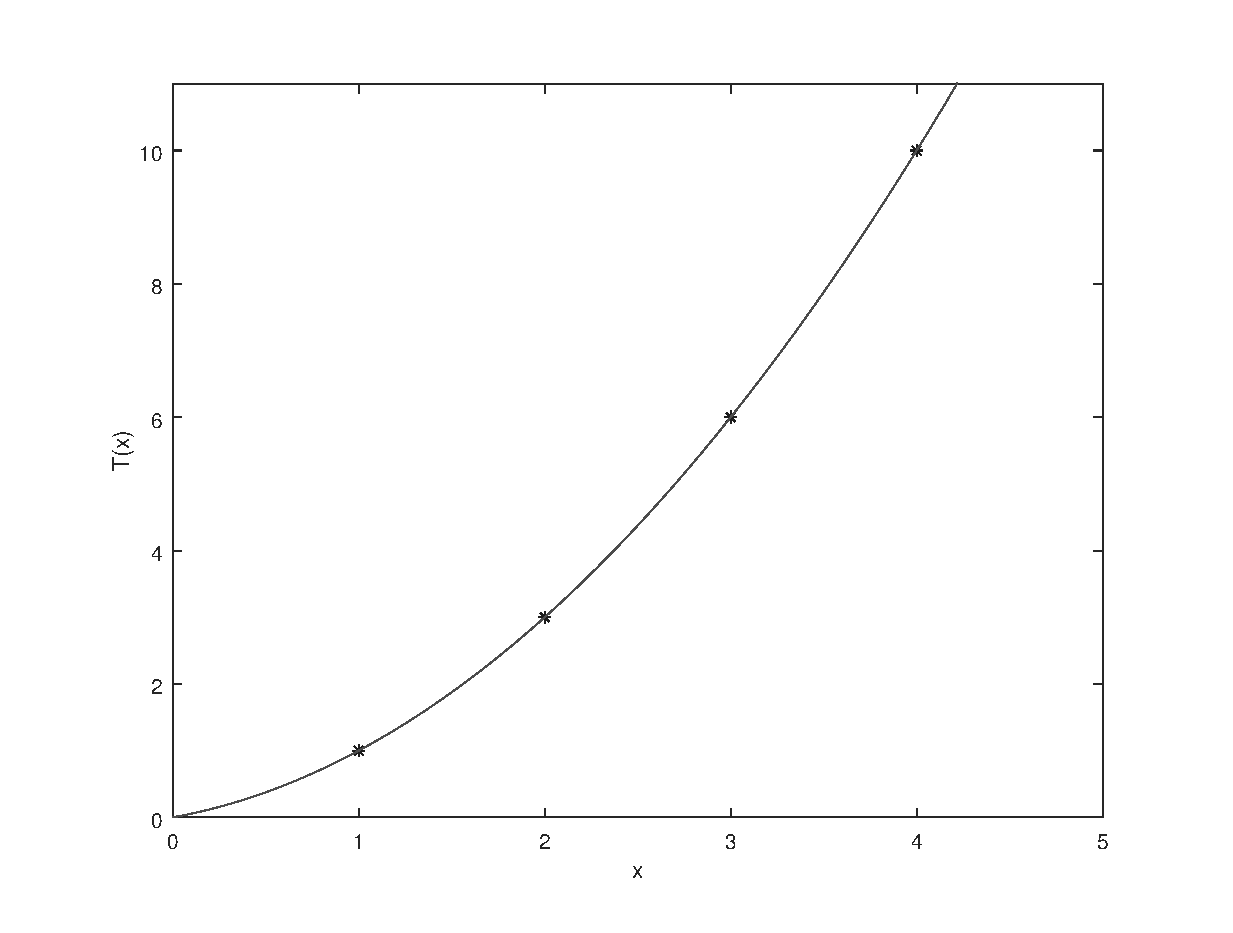
\includegraphics[scale=0.5]{figura1_2.eps}
	\end{center}
\caption{Interpolación de los números triangulares}
\label{fig1_2}
\end{figure}
\begin{figure}[htbp]
	\begin{center}
		\includegraphics[scale=0.5]{figura1_3.eps}
	\end{center}
\caption{Secuencia de números factoriales}
\label{fig1_3}
\end{figure}

Ahora, para iniciar con el estudio de la función gamma, se define de una manera formal la función factorial.
\begin{definition}
	Sea $n \in \mathbb{N}$, entonces la función factorial se define como $$n! = \prod_{k=1}^{n} k.$$
\end{definition}

Determinando así que $n!$ es el producto de los $n$ primeros números naturales. ¿Qué pasa con $0!$? Si volvemos a nuestros números triangulares, vemos que se cumple esta relación de recurrencia $$T_{n+1} = T_n + (n+1).$$ Si hacemos $n = 0$, obtenemos que $T_0 = 0.$ Así, $0$ sería un tipo de número triangular y esto, nos conlleva a la definición de suma vacía y producto vacío. 

\begin{definition}
		Sea $K$ un cuerpo y sean $a_k \in K$ con $k = 1,\ 2,\ 3,\ \dots,\ n$. Entonces para el conjunto $\{k \in \mathbb{N}\ :\ k\leq n\}$, $$\sum_{k>n} a_k = 0, \hspace{1cm} \prod_{k>n} a_k = 1.$$
\end{definition}

Lo anterior es resultado de que si $S_n = \sum_{k=1}^{n} a_k$ y $P_n = \prod_{k=1}^{n} a_k$ con $n \in \mathbb{N},$ entonces
$$S_{n+1} = a_{n+1}+S_n, \hspace{1cm} P_{n+1} = a_{n+1}P_n.$$
Como $S_1 = a_1$ y $P_1 = a_1$, podemos usar las expresiones anteriores con $n = 0$ y llegar a $S_0 = 0$ y $P_0 = 1,$ que corresponden a los elementos neutros de la suma y el producto del cuerpo. Luego, usando la definición 1.1, $0! = 1.$ Además, como $$n! = n \prod_{k=1}^{n-1} k,$$ entonces se llega a la fórmula de recurrencia del factorial
\begin{equation}
	n! = \left\{ \begin{array}{rcl}
	n(n-1)! & \mbox{para} & n\geq1\\
	&				&\\
	1 & \mbox{para} & n = 0.\\
	\end{array}\right.
\end{equation}

\section{El nacimiento de la función gamma de Euler}

En la sección anterior vimos que para la secuencia de números triangulares, se puede encontrar una fórmula general que funcione para todo $x \in \mathbb{R}$, la cual, cuando $x = n \in \mathbb{N}$, genere el $n$-ésimo número triangular correspondiente. Para la secuencia de números factoriales, Euler encontró que la fórmula
\begin{equation}
	n! = \int_{0}^{1}\, (-\ln t)^n\, dt, 
\end{equation}
genera valores numéricos para números diferentes a los enteros no negativos y, para el caso en que $n \in \mathbb{Z}_0^+,$ genera los números factoriales. En la Figura \ref{fig1_4} vemos cómo la fórmula (1.3) interpola los términos factoriales. 

Cabe destacar, que la fórmula (1.1) solo me genera números triangulares cuando $x = n \in\mathbb{N},$ porque para valores distintos pierde su significado original. Igualmente sucede con los números factoriales y la expresión (1.3), ya que $(1/2)!$ no es una expresión factorial. De hecho, encontramos extensiones de tales expresiones en $\mathbb{R}$, que al restringir su dominio a $\mathbb{Z}_0^+$ me generan números triangulares y factoriales respectivamente. De manera similar sucede con la suma infinita de todos los números naturales $$\sum_{k=1}^{\infty}\ k = -\frac{1}{12},$$ que se encuentra en Berndt (1985). Esta identidad no es completamente cierta, ya que la parte izquierda de la igualdad es una serie divergente, pero representa un hecho muy interesante relacionado con la función zeta de Riemann. Este resultado se explica con más detalle en el capítulo 4 del presente trabajo. 

\begin{figure}[htbp]
	\begin{center}
		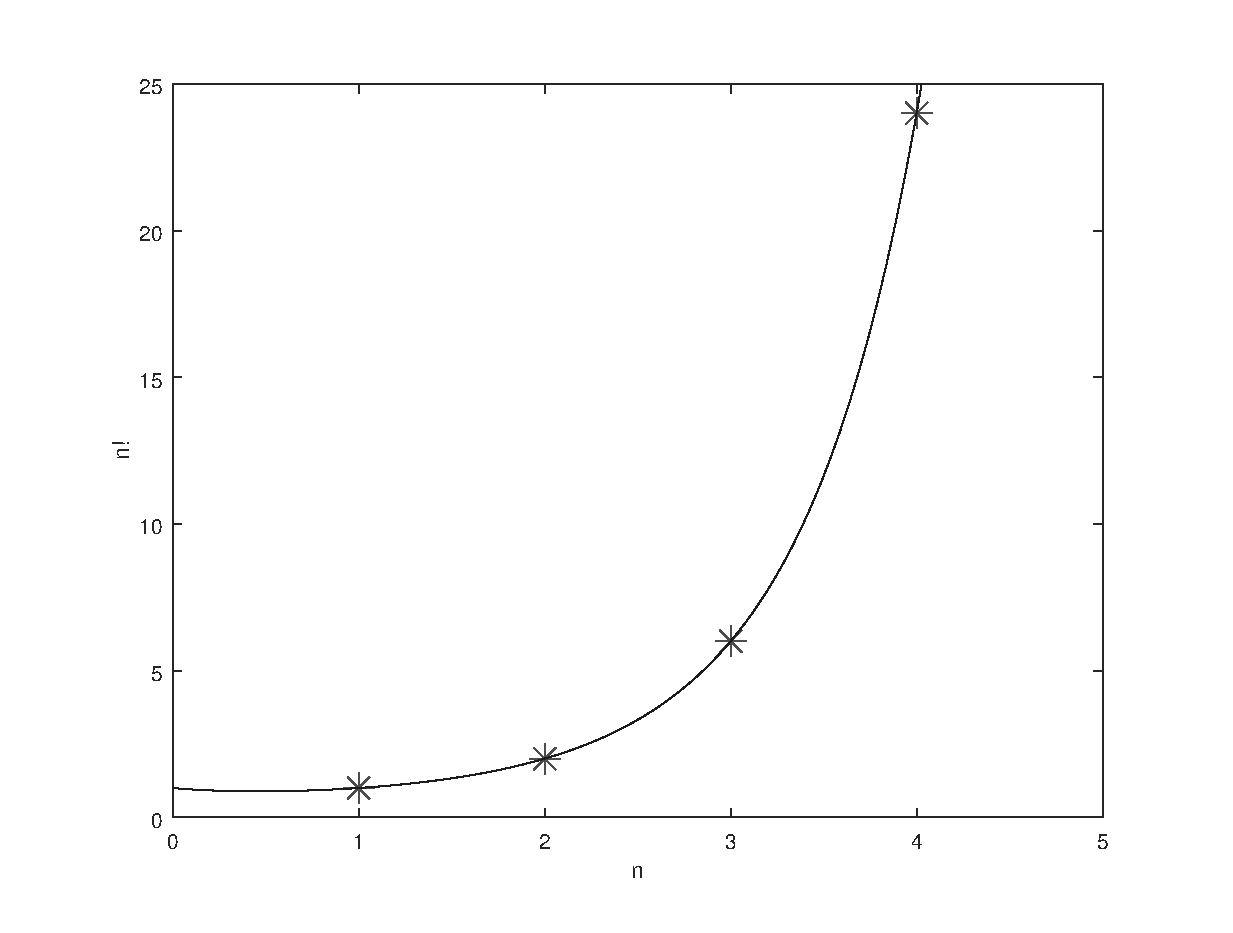
\includegraphics[scale=0.5]{figura1_4.eps}
	\end{center}
\caption{Interpolación de los números factoriales}
\label{fig1_4}
\end{figure}

El 13 de octubre de 1729, Euler en una carta escrita a Goldbach resuelve el problema de la función factorial, concluyendo que no era posible encontrar una fórmula algebraica sencilla. La fórmula que encontró consta de términos infinitos y, respondiendo a lo referente con la interpolación de números factoriales, interpola cualquier par de términos factoriales. La fórmula a la que llegó es el famoso producto infinito de Euler, 
\begin{equation}
	x! = \lim\limits_{n\rightarrow\infty} \frac{n!\ n^x}{\prod_{k=1}^{n}(x+k)}\ \textrm{para}\ x\in \mathbb{R}\texttt{\textbackslash}\mathbb{Z}^-.
\end{equation}

Euler, al comprobar que su fórmula generaba los números factoriales correspondientes, ingresa un número fraccionario, $1/2$, obteniendo $$(1/2)! = {\sqrt{\pi} \over 2}.$$ Tal resultado inesperado condujo a Euler a pensar en la existencia de una relación con una fórmula integral, ya que involucraba la cuadratura de una circunferencia unitaria. Euler (1738), comenta que su producto infinito es muy poco práctico para hallar términos factoriales. Que al ver la secuencia detenidamente de los números factoriales, pensó que tenían un comportamiento exponencial, pero al ver el resultado obtenido con el número $1/2$, descartó tal idea.

El 8 de enero de 1730, en respuesta a la carta enviada por Goldbach del 1ro de diciembre de 1729, Euler encuentra con éxito la fórmula integral que estaba buscando, la integral impropia (1.3). Tiempo después, en el año 1738, publica su artículo "\textit{De progressionibus transcendentibus seu quarum termini generales algebraice dari nequeunt}", donde expone de manera más detallada los resultados expuestos en las 2 cartas. Luego, en el año 1809, el matemático francés Adrien-Marie Legendre (1752-1833) nombró a la expresión factorial de Euler $(x-1)!$ (integral de Euler de segunda especie) como la función gamma de Euler, dándole su símbolo representativo $\Gamma,$ $$\Gamma(z) = \int_{0}^{\infty}t^{z-1}e^{-t}\ dt,\ \textrm{donde}\ Re(z)>0.$$

La integral de Euler de primera especie estaba definida por $$\int_{0}^{1} x^m\ (1-x)^n\ dx,$$ la cual fue determinante en la deducción de la integral de segunda forma. Tiempo después, el matemático francés Jacques Philippe Marie Binet (1786-1856), reconocido por su fórmula explícita de los términos de la sucesión de Fibonacci, le dio el nombre de función beta. La cual se representa como $$B(z,w) = \int_{0}^{1} t^{z-1}\ (1-t)^{w-1}\ dt,\ \textrm{para}\ Re(z)>0, Re(w)>0.$$

Como el simple deseo de extender la función factorial a valores que estén entre los enteros positivos llevó al descubrimiento de la función gamma, el deseo de extenderla a valores negativos y a los números complejos, llevó a su desarrollo más completo y a una interpretación más profunda. Si intentamos extendernos a los enteros negativos $\mathbb{Z}^-$, por ejemplo, hallando el factorial de $-2,$ de manera heurística nos encontraríamos con un comportamiento divergente. $$(-2)! = (-2)(-3)(-4)(-5)\cdot\dots$$ 

Si se observa el producto infinito de Euler (1.4), no sería posible hallar el factorial de un número entero negativo, ya que en algún momento se anularía el denominador en esa expresión. Además, como generalización de la propiedad $n! = n(n-1)!$ se tiene la fórmula de recurrencia 
\begin{equation}
	x\ \Gamma(x) = \Gamma(x+1),\ x>0.
\end{equation} 
Esta es una relación útil y práctica para evaluar el factorial de un número real positivo cualquiera hallando el factorial de un número apropiado entre $0$ y $1.$ Así, para $n = 5\ {1 \over 2},$ se tiene $$\left(5\ \tfrac{1}{2}\right)! = \left(5\ \tfrac{1}{2}\right)\left(4\ \tfrac{1}{2}\right)\left(3\ \tfrac{1}{2}\right)\left(2\ \tfrac{1}{2}\right)\left(1\ \tfrac{1}{2}\right)\left(\tfrac{1}{2}\right)!,$$ y como $(1/2)! = \frac{\sqrt{\pi}}{2},$ entonces $$\left(5\ \tfrac{1}{2}\right)! = \left(\frac{3\cdot5\cdot7\cdot9\cdot11}{2^6}\right)\sqrt{\pi}.$$
 
En los primeros años del siglo XIX, se trató la función factorial en el plano complejo. Este traslado de la recta real al plano complejo fue iniciado por el matemático alemán Carl Friedrich Gauss (1777-1855), quien comenzó con el producto de Euler, $$\Pi(z) = \lim\limits_{n\rightarrow\infty} \frac{n!\ n^z}{\prod_{k=1}^{n}(z+k)}\ \textrm{para}\ z \neq -1,\ -2,\ -3,\ \dots$$

Luego, los matemáticos alemanes Bernhard Riemann (1826-1866) y Karl Weierstrass (1815-1897), usando la relación de recurrencia $\Gamma(z+1) = z\ \Gamma(z),$ extendieron el dominio de la función gamma a los complejos caracterizando la función $1/\Gamma(z).$ Además, Riemann trabajó su función zeta relacionándola con la función gamma. En 1876, Weierstrass tuvo éxito en producir una teoría extensiva de factorización de funciones, la cual incluía como casos especiales los conocidos productos infinitos, así como funciones doblemente periódicas. Gracias a esto, Weierstrass dedujo el producto infinito de $1/\Gamma(z),$ el cual mostraba de manera explícita los ceros de la función $1/\Gamma(z).$

Vemos que la función gamma cumple con que $\Gamma(1) = 1.$ Cumple también la relación de recurrencia (1.5) y es analítica cuando $x>0.$ Pero, ¿será la única función que cumple las condiciones anteriores y que genere números factoriales al evaluarla en los enteros positivos? Si probamos con la función $p(x) = 1+\sin 2\pi x$ multiplicándola con la función gamma, el resultado sería una función analítica para $x>0,$ que satisface la relación de recurrencia (ya que $p(x)$ es de período $1$), y produce términos factoriales. Se necesitaba una condición fuerte que pudiera determinar la unicidad de la función gamma.

A finales del siglo XIX e inicios del siglo XX, la teoría de funciones tomó un rumbo muy diferente, respaldada por la teoría de conjuntos de Cantor y una emergente teoría topológica. La nueva teoría de funciones no se fijó mucho en ecuaciones ni en identidades, pero sí en las propiedades geométricas fundamentales. Así, la condición deseada fue encontrada en la noción de convexidad. Una curva es convexa si tomando dos puntos de ella y uniéndolos con una línea recta, la porción de curva entre los puntos yace abajo de la recta, Davis (1959). Vemos en la Figura \ref{fig1_5} que las curvas individuales generadas de la función gamma que están en el primer y segundo cuadrante son todas convexas. 

\begin{figure}[htbp]
	\begin{center}
		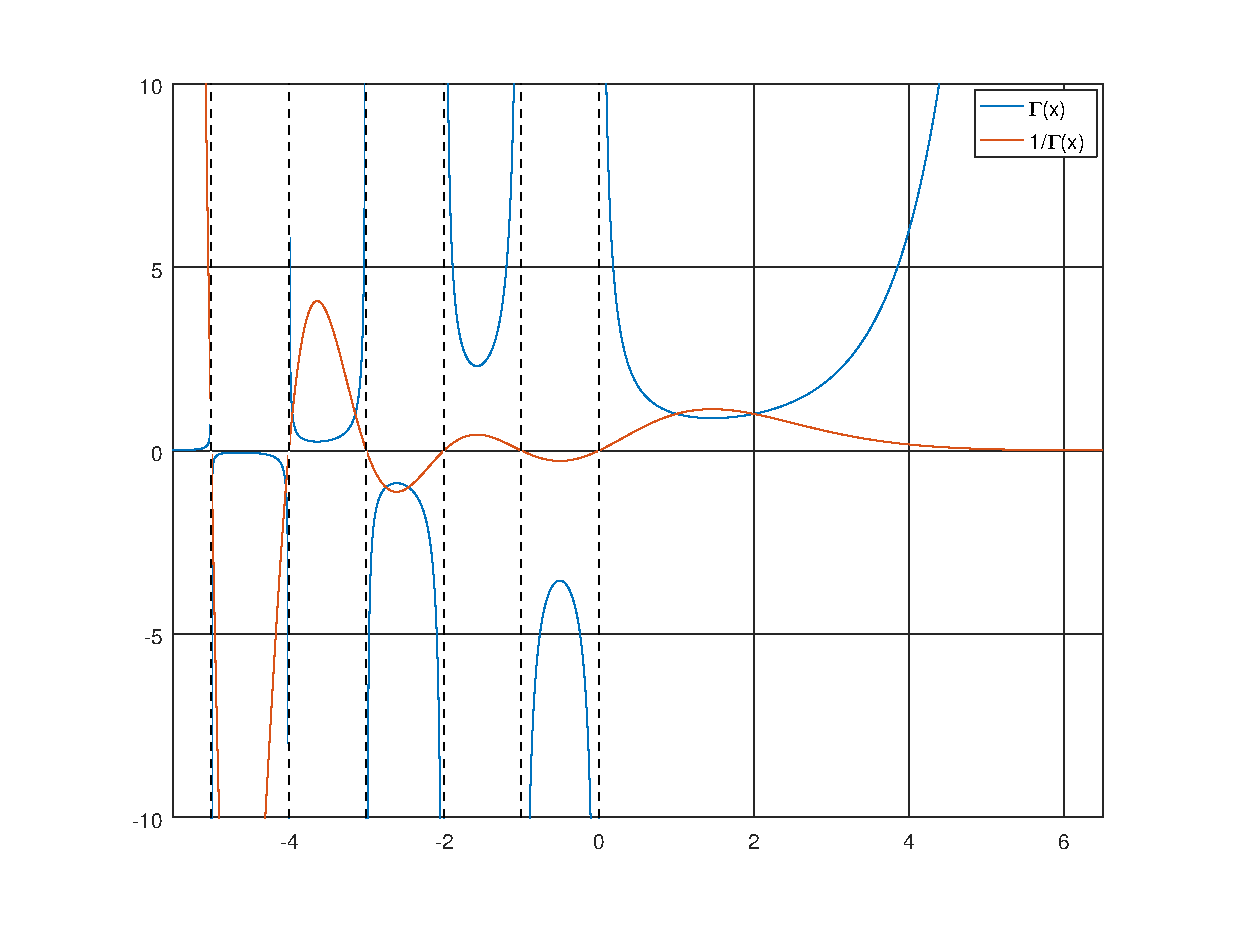
\includegraphics[scale=0.7]{figura1_5.eps}
	\end{center}
\caption{Función gamma y función gamma inversa}
\label{fig1_5}
\end{figure}

Ahora, ¿la función gamma es la única función que genera valores factoriales, satisface la relación de recurrencia y es convexa para $x>0$? Si consideramos la función "pseudo" gamma $\emph{G}_s(x),$ la cual se construye de la siguiente manera 
\begin{align*}
	\emph{G}_s(x) &= 1/x \hspace{1cm}\ &0 < x \leq 1 \\
	\emph{G}_s(x) &= 1				&1 < x \leq 2\\
	\emph{G}_s(x) &= x-1 				&2 < x \leq 3\\
	\emph{G}_s(x) &= (x-1)(x-2)		&3 < x \leq 4\\
	\vdots
\end{align*}
y que está representada en la Figura \ref{fig1_6},
\begin{figure}[htbp]
	\begin{center}
		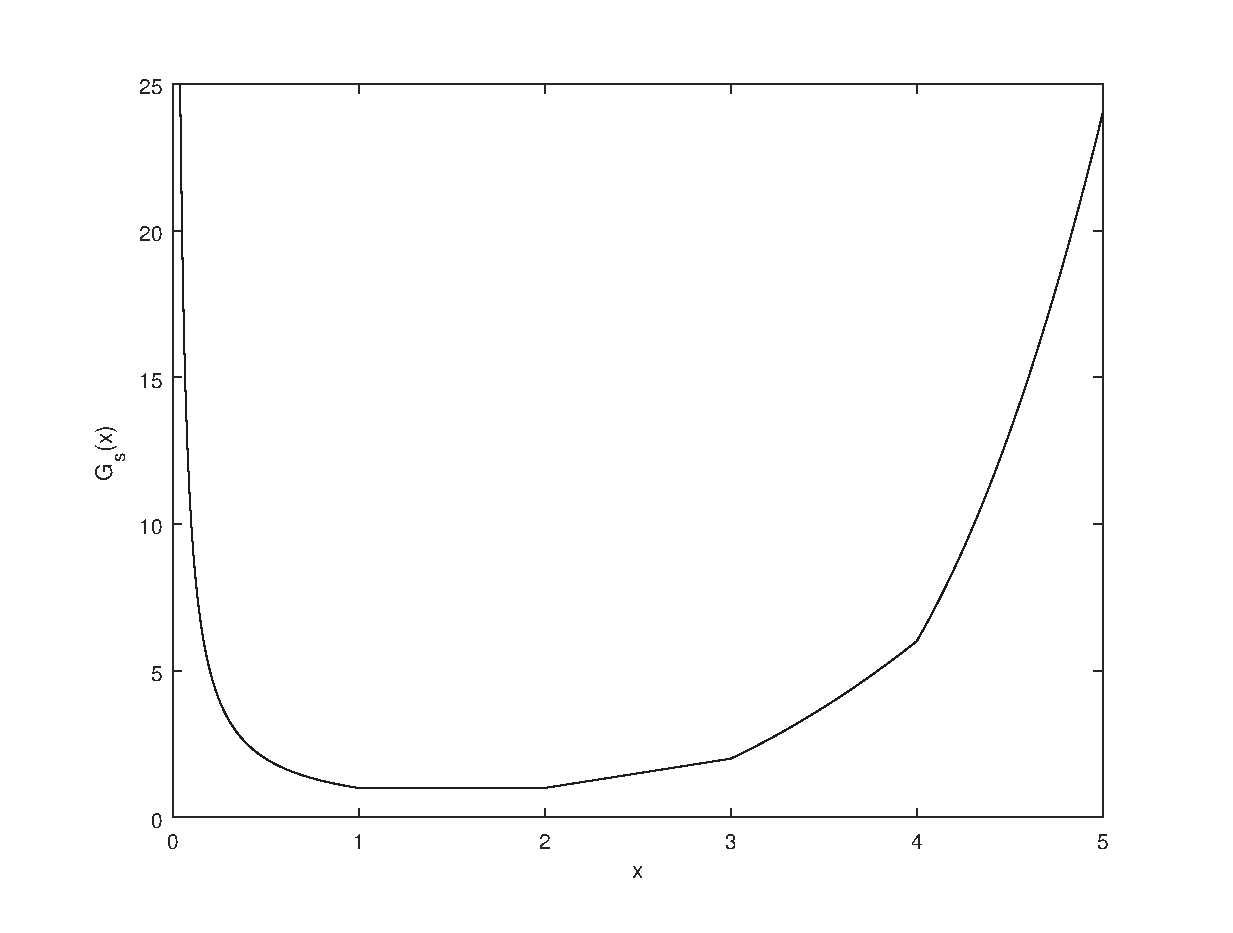
\includegraphics[scale=0.5]{figura1_6.eps}
	\end{center}
\caption{Función pseudogamma}
\label{fig1_6}
\end{figure}
vemos que esta función cumple las condiciones anteriormente discutidas. Se necesita una condición más fuerte, como la de convexidad logarítmica, para poder llegar a caracterizar eficientemente a la función gamma. Podemos ver en la Figura \ref{fig1_7} que la curva del logaritmo de la función gamma es convexa, así, la función gamma es logarítmicamente convexa. En este momento, nos encontramos con el famoso teorema de Bohr-Mollerup, que fue enunciado y demostrado por los matemáticos daneses Harald Bohr (1887-1951) y Johannes Mollerup (1872-1937) en el año 1922. El teorema afirma que la única función que cumple que para $x>0,$ $f(1) = 1,$ sea logarítmicamente convexa y que cumpla con la fórmula de recurrencia $f(x+1) = xf(x),$ es la función gamma de Euler.
\begin{figure}[htbp]
	\begin{center}
		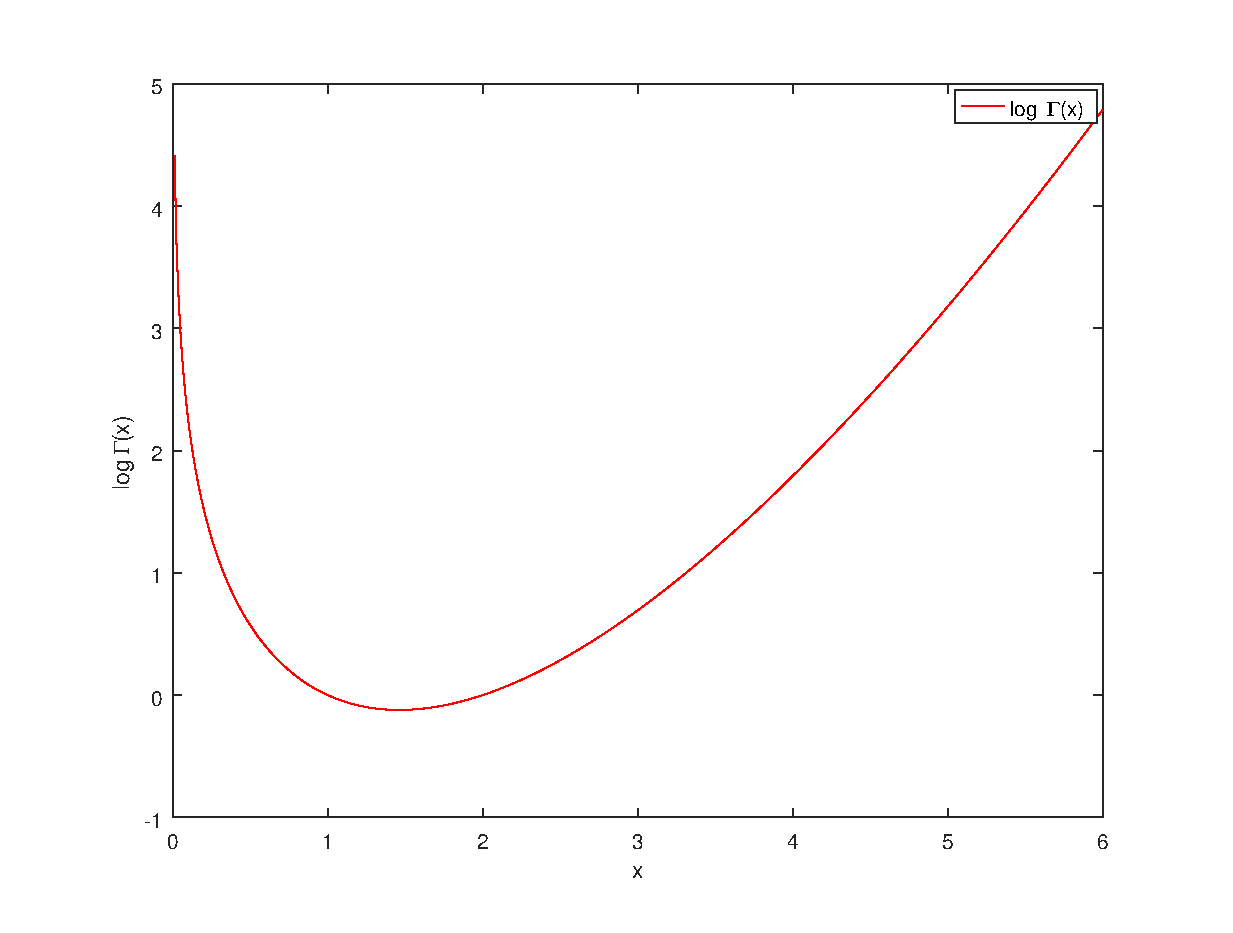
\includegraphics[scale=0.5]{figura1_7.eps}
	\end{center}
\caption{Logaritmo de la función gamma}
\label{fig1_7}
\end{figure}

Para terminar este capítulo, se hace un esbozo muy poco formal del desarrollo de la función gamma hasta la forma integral definida por Legendre. Primero, se parte de la expresión (1.2) y se procede de manera similar a la realizada en Andrews (1999) y Davis (1959). En lo que resta de este capítulo y en el capítulo 2, se necesitan conocimientos de cálculo en la recta real que abarquen convergencia de sucesiones y de series, continuidad, convergencia de sucesiones de funciones, diferenciabilidad e integrabilidad, los cuales Apostol (1967), Arens (2013), Fischer (1983), Little (2015) y Ross (2013) serían de gran utilidad para el lector.

Para $x, n \in \mathbb{Z}_0^+$ con $n>0,$ tenemos que $$(x+n)! = n!\ \prod_{k=1}^{x}(n+k),$$ y además $$(x+n)! = x!\ \prod_{k=1}^{n}(x+k).$$ Por lo anterior, se puede reescribir $x!$ de la siguiente manera
\begin{align*}
	x! &= \frac{x!\prod_{k = 1}^{n}(x+k)}{\prod_{k = 1}^{n}(x+k)} \\
	&= \frac{(x+n)!}{\prod_{k=1}^{n}(x+k)} \\
	&= \frac{n!\ \prod_{k=1}^{x}(n+k)}{\prod_{k=1}^{n}(x+k)} \\
	&= \frac{n!\ n^x}{\prod_{k=1}^{n}(x+k)}\cdot\frac{\prod_{k=1}^{x}(n+k)}{n^x},
\end{align*}
y haciendo $n\rightarrow\infty$, llegamos a que
\begin{align*}
	\lim_{n\rightarrow\infty} x! &= \lim_{n\rightarrow\infty} \left[\frac{n!\  n^x}{\prod_{k=1}^{n}(x+k)}\cdot\frac{\prod_{k=1}^{x}(n+k)}{n^x}\right] \\
	x! &= \lim_{n\rightarrow\infty} \frac{n!\ n^x}{\prod_{k=1}^{n}(x+k)} \cdot \lim_{n\rightarrow\infty} \frac{(n+1)(n+2)\cdot...\cdot(n+x)}{n^x}  \\
	&= \lim_{n\rightarrow\infty} \frac{n!\ n^x}{\prod_{k=1}^{n}(x+k)} \cdot \lim_{n\rightarrow\infty} \left[\left(\frac{n+1}{n}\right)\left(\frac{n+2}{n}\right)\cdot...\cdot\left(\frac{n+x}{n}\right)\right]  \\
	&= \lim_{n\rightarrow\infty} \frac{n!\ n^x}{\prod_{k=1}^{n}(x+k)} \cdot \lim_{n\rightarrow\infty} \left(1+\tfrac{1}{n}\right)\cdot \lim_{n\rightarrow\infty} \left(1+\tfrac{2}{n}\right)\cdot ...\cdot \lim_{n\rightarrow\infty} \left(1+\tfrac{x}{n}\right) \\
	&= \lim_{n\rightarrow\infty} \frac{n!\ n^x}{\prod_{k=1}^{n}(x+k)}.
\end{align*}
Si hacemos $x = 0,$ se obtiene el cociente $n!/n!,$ y así la fórmula se verifica para $x = 0.$ Además, también lo hace para cualquier valor $m \in \mathbb{N},$ aunque no sea muy práctica para hallar tales términos. Veamos, que para $m \in \mathbb{N}$ se tiene que
\begin{align*}
	m! &= \lim_{n \rightarrow \infty} \frac{n!\ n^m}{\prod_{k=1}^{n}(m+k)}\\
		&= \lim_{n \rightarrow \infty} \frac{(\prod_{k=1}^{n}k)\cdot n^m}{\prod_{k=1}^{n}(m+k)}\\
		&= 	\lim_{n \rightarrow \infty} \frac{m!\cdot(\prod_{k=1}^{n-m}(m+k))\cdot n^m}{(\prod_{k=1}^{n-m}(m+k))\cdot(\prod_{k=1}^{m}(n+k))}\\
		&= m!\cdot \lim_{n \rightarrow \infty} \left(\frac{n}{n+1}\cdot\frac{n}{n+2}\cdot\ \dots\ \cdot\frac{n}{n+m}\right)\\
		&= m!
\end{align*}
Ahora, si tomamos $x = 1/2,$ entonces
\begin{align*}
(1/2)! &= \lim_{n \rightarrow \infty}\frac{n!\ \sqrt{n}}{\prod_{k = 1}^{n}\left(\frac{1}{2}+k\right)} \\
&= \lim_{n \rightarrow \infty}\frac{2^n n!\ \sqrt{n}}{\prod_{k = 1}^{n}(2k+1)} \\
&= \lim_{n \rightarrow \infty} \left[\frac{2 \cdot 4 \cdot 6 \cdot 8 \cdot ... \cdot (2n)}{3 \cdot 5 \cdot 7 \cdot 9 \cdot ... \cdot (2n+1)} \sqrt{n}\right] \\
&= \lim_{n \rightarrow \infty}\left[\frac{2 \cdot 4 \cdot 6 \cdot 8 \cdot ... \cdot (2n)}{1 \cdot 3 \cdot 5 \cdot 7 \cdot ... \cdot (2n-1)}\cdot \frac{\sqrt{n}}{(2n+1)}\right], \\
\intertext{y elevando al cuadrado, se obtiene}
[(1/2)!]^2 &= \lim_{n \rightarrow \infty} \left[\frac{2 \cdot 2 \cdot 4 \cdot 4 \cdot 6 \cdot 6 \cdot 8 \cdot 8 \cdot ... \cdot (2n)(2n)}{1 \cdot 1 \cdot 3 \cdot 3 \cdot 5 \cdot 5 \cdot 7 \cdot 7 \cdot ... \cdot (2n-1)(2n-1)}\cdot \frac{n}{(2n+1)^2}\right]  \\
&= \lim_{n \rightarrow \infty} \left[\frac{2 \cdot 2 \cdot 4 \cdot 4 \cdot 6 \cdot 6 \cdot 8 \cdot 8 \cdot ... \cdot (2n)(2n)}{1 \cdot 3 \cdot 3 \cdot 5 \cdot 5 \cdot 7 \cdot 7 \cdot 9 \cdot ... \cdot (2n-1)(2n+1)}\cdot \frac{n}{(2n+1)}\right]  \\
&= \lim_{n \rightarrow \infty} \frac{2 \cdot 2 \cdot 4 \cdot 4 \cdot 6 \cdot 6 \cdot 8 \cdot 8 \cdot ... \cdot (2n)(2n)}{1 \cdot 3 \cdot 3 \cdot 5 \cdot 5 \cdot 7 \cdot 7 \cdot 9 \cdot ... \cdot (2n-1)(2n+1)}\cdot \lim_{n \rightarrow \infty} \frac{n}{(2n+1)} \\
&= \frac{1}{2}\cdot \lim_{n \rightarrow \infty} \frac{2 \cdot 2 \cdot 4 \cdot 4 \cdot 6 \cdot 6 \cdot 8 \cdot 8 \cdot ... \cdot (2n)(2n)}{1 \cdot 3 \cdot 3 \cdot 5 \cdot 5 \cdot 7 \cdot 7 \cdot 9 \cdot ... \cdot (2n-1)(2n+1)} \\
&= \frac{1}{2}\cdot \prod_{k = 1}^{\infty}\ \left(\frac{2k}{2k-1}\cdot\frac{2k}{2k+1}\right).
\end{align*}

El producto infinito resultante se conoce como el producto de Wallis. El matemático inglés John Wallis (1616-1703) descubrió que este producto es igual a $\frac{\pi}{2}$ en el año 1656. A continuación se realiza la deducción de esta fórmula siguiendo la demostración hecha en Hijab (2016).
Vemos que $\forall n\in \mathbb{Z}_0^+$ tal que $n\geq2$ se tiene, $$\int\sin^n x\ dx = \int\sin^{n-1} x \ \sin x \ dx$$
Integrando por partes, se llega a
\begin{equation}
	\int\sin^n x \ dx = -{1 \over n}\sin^{n-1} x \ \cos x +\frac{n-1}{n}\int\sin^{n-2} x \ dx.
\end{equation}
Ahora, evaluando de $0$ a $\pi/2,$ $$\int_{0}^{\pi/2}\sin^n x\ dx = \frac{n-1}{n}\int_{0}^{\pi/2}\sin^{n-2} x \ dx.$$
Como $\int_{0}^{\pi/2} \ dx = {\pi \over 2}$ y $\int_{0}^{\pi/2}\sin x \ dx = 1,$ entonces usando (1.6) para $n\geq2,$ $$\int_{0}^{\pi/2}\sin^2 x \ dx = {1 \over 2}\cdot{\pi \over 2}, \hspace{0.5cm}\int_{0}^{\pi/2}\sin^3 x \ dx = {2 \over 3}\cdot 1,\ \dots$$
Por inducción matemática llegamos a las fórmulas siguientes,
\begin{align*}
	I_{2n} &= \int_{0}^{\pi/2}\sin^{2n} x \ dx = \frac{1}{2}\cdot\frac{3}{4}\cdot\ \dots\ \cdot \frac{2n-3}{2n-2}\cdot\frac{2n-1}{2n}\cdot\frac{\pi}{2}, \ \forall n \in \mathbb{N}\\
	I_{2n+1} &= \int_{0}^{\pi/2}\sin^{2n+1} x \ dx = \frac{2}{3}\cdot\frac{4}{5}\cdot\ \dots\ \cdot \frac{2n-2}{2n-1}\cdot\frac{2n}{2n+1}\cdot 1, \ \forall n \in \mathbb{N}.
\end{align*}
Como $0\leq\sin x \leq1$ en $[0,\pi/2],$ entonces $$0\leq\sin^n x \leq\sin^{n-1} x ,\hspace{0.5 cm}\forall n\geq 1.$$
Además, por propiedad monótona de la integral, $$0 \leq \int_{0}^{\pi/2}\sin^n x \ dx \leq \int_{0}^{\pi/2}\sin^{n-1} x \ dx,\hspace{0.5cm} \forall n\geq 1.$$
Así, $$I_{2n+1}\leq I_{2n}\hspace{0.5cm} \textrm{y} \hspace{0.5cm}I_{2n}\leq I_{2n-1}.$$
Como $$\frac{I_{2n-1}}{I_{2n+1}} = \frac{2n+1}{2n},$$ entonces $$1\leq\frac{I_{2n}}{I_{2n+1}}\leq \frac{I_{2n-1}}{I_{2n+1}} = \frac{2n+1}{2n}.$$
Cuando $n\rightarrow\infty,$ $$\frac{I_{2n}}{I_{2n+1}}\rightarrow\ 1$$ por propiedad de estricción (teorema del emparedado).

Además, tenemos que $$\frac{I_{2n+1}}{I_{2n}} = \frac{2}{\pi}\cdot\frac{2\cdot2\cdot4\cdot4\cdot\ \dots\ \cdot(2n-2)(2n-2)(2n)(2n)}{1\cdot3\cdot3\cdot5\cdot\ \dots\ \cdot(2n-3)(2n-1)(2n-1)(2n+1)},$$ entonces
$$\frac{\pi}{2} = \frac{I_{2n}}{I_{2n+1}}\cdot\frac{2\cdot2\cdot4\cdot4\cdot\ \dots\ \cdot(2n-2)(2n-2)(2n)(2n)}{1\cdot3\cdot3\cdot5\cdot\ \dots\ \cdot(2n-3)(2n-1)(2n-1)(2n+1)}$$ y haciendo $n\rightarrow\infty$ llegamos al siguiente resultado $$\lim_{n \rightarrow \infty}\ \frac{2\cdot2\cdot4\cdot4\cdot\ \dots\ \cdot(2n)(2n)}{1\cdot3\cdot3\cdot5\cdot\ \dots\ \cdot(2n-1)(2n+1)} = \frac{\pi}{2},$$ que en otras palabras es $$\prod_{k = 1}^{\infty}\ \left(\frac{2k}{2k-1}\cdot\frac{2k}{2k+1}\right) = \frac{\pi}{2}.$$ Por lo anterior  $$\left({1 \over 2}\right)! = {\sqrt{\pi}\over 2},$$ 
así que la expresión (1.4) es válida, en lo que respecta al tratamiento heurístico que se está abordando.
 
Por último, se deduce (1.3) a partir de la integral de Euler de primera especie, tomando como base a Euler (1738) y a Andrews (1999). Luego, llegamos a la representación de Legendre siguiendo a Andrews (1999) y a Davis (1959). Pero antes de realizar tal procedimiento preguntémonos, ¿por qué la integral de Euler de primera especie? Aunque Euler no lo mencionó de manera explícita, el hecho de que $(1/2)! = \sqrt{\pi}/2$ pudo haberlo animado a usar la integral $$\int_{0}^{1}\sqrt{1-x^2}\ dx = \int_{0}^{1}(1+x)^{1/2}\ (1-x)^{1/2}\ dx = \frac{\pi}{4},$$ la cual representa el área de la cuarta parte del círculo unitario. Vemos que tal expresión posee alguna similitud con la integral de primera especie, donde $n = 1/2$ arroja una pista para la deducción de la integral de segunda especie.

Así, usando el teorema del binomio de Newton con $n \in \mathbb{Z}_0^+$ en la integral de Euler de primera especie $$\int_{0}^{1}x^m\ (1-x)^n\ dx,$$ obtenemos
\begin{align*}
	\int_{0}^{1} x^m\ (1-x)^n\ dx = \sum_{k = 0}^{n}\binom{n}{k}(-1)^k\frac{1}{m+k+1}.
\end{align*}
Por consiguiente, para $n = 0$ llegamos a $$\int_{0}^{1}x^m\ dx = \frac{1}{m+1},$$
para $n = 1$
$$\int_{0}^{1}x^m\ (1-x)\ dx = \frac{1}{m+1} - \frac{1}{m+2} = \frac{1}{(m+1)(m+2)},$$
para $n = 2$
$$\int_{0}^{1}x^m\ (1-x)^2\ dx = \frac{1}{m+1} - \frac{2}{m+2} + \frac{1}{m+3} = \frac{1 \cdot 2}{(m+1)(m+2)(m+3)},$$
y así por inducción matemática, usando integración por partes, obtenemos la expresión $$\int_{0}^{1}x^m\ (1-x)^n\ dx = \frac{n!}{(m+1)(m+2)(m+3) \cdot \ldots \cdot (m+n+1)},$$ para $n \in \mathbb{Z}_0^+.$

Si $m = f/g,$ donde $f,g \in \mathbb{Z}_0^+$ con $g \neq 0,$ entonces
$$\frac{n!}{(f+g)(f+2g) \cdot \ldots \cdot (f+ng)} = \frac{f+(n+1)g}{g^{n+1}}\int_{0}^{1}x^{f/g}(1-x)^n\ dx,$$ haciendo $x = t^{\frac{g}{f+g}}$ tenemos que
$$\frac{n!}{(f+g)(f+2g) \cdot \ldots \cdot (f+ng)} = \frac{f+(n+1)g}{(f+g)^{n+1}}\int_{0}^{1}\left(\frac{1-t^{\frac{g}{f+g}}}{\tfrac{g}{f+g}}\right)^n\ dt.$$ Si $f = 1$ y $g = 0,$ entonces $k = \frac{g}{f+g} = 0,$ usando la regla de l'Hôpital llegamos a $$\lim_{k \rightarrow 0} \frac{1-t^k}{k} = -\ln t,$$ y así
$$n! = \int_{0}^{1}\ (-\ln t)^n\ dt.$$

La integral de Euler es válida para todo número positivo, y en el momento fue conocida como la integral de Euler de segunda especie, Davis (1959). Legendre, partiendo de la expresión $$(n-1)! = \int_{0}^{1}\ (-\ln x)^{n-1}\ dx,$$ dedujo lo que hoy se conoce como la función gamma de Euler por medio del cambio de variable $$t = -\ln x.$$ Como la función $\ln$ es creciente, entonces
$$(n-1)! = \int_{\infty}^{0}\ t^{n-1}\ (-x)\ dt = \int_{0}^{\infty}\ t^{n-1}\ x\ dt,$$ y utilizando el cambio de variable, donde $x = e^{-t},$ obtenemos $$(n-1)! = \int_{0}^{\infty}\ t^{n-1}\ e^{-t}\ dt.$$ Finalmente, llegamos a la representación clásica de la función gamma de Euler, definida por Legendre de la siguiente manera, $$\Gamma (x) = \int_{0}^{\infty}\  e^{-t}\ t^{x-1}\ dt,\ \textrm{para}\ x \in \mathbb{R}_{>0}.$$
\endinput
%La función gamma en R
%
\chapter{La función gamma en $\mathbb{R}$}
\addcontentsline{lof}{chapter}{2. La función gamma en $\mathbb{R}$}
Luego de una corta introducción histórica al desarrollo de la función gamma de Euler, en el presente capítulo llegamos a determinar por medio del teorema de Bohr-Mollerup, la existencia y unicidad de dicha "generalización" del factorial en la recta real. Siguiendo el tratamiento hecho por Artin (1961) y Fischer (1983), podemos demostrar dicho teorema usando el concepto de convexidad logarítmica. Gracias a este concepto, se llega a una caracterización de la función gamma por medio de la definición de su dominio en $\mathbb{R},$ junto con la prueba de su continuidad en dicho dominio. Luego de la demostración del teorema de Bohr-Mollerup, se exponen junto con el producto de Euler, la representación integral y el producto de Weierstrass en $\mathbb{R},$ los cuales son retomados en el capítulo siguiente. 

\section{Convexidad y convexidad logarítmica}
De manera similar al concepto manejado en el capítulo anterior, una función es convexa cuando la recta secante formada por los puntos $P_1 = (x,f(x))$ y $P_2 = (y,f(y))$ se encuentra por encima de la curva que está suspendida entre tales puntos, como vemos en la figura \ref{fig2_1}. Para llegar a una definición más formal, primero definiremos qué es un conjunto convexo.

\begin{figure}[htbp]
	\begin{center}
		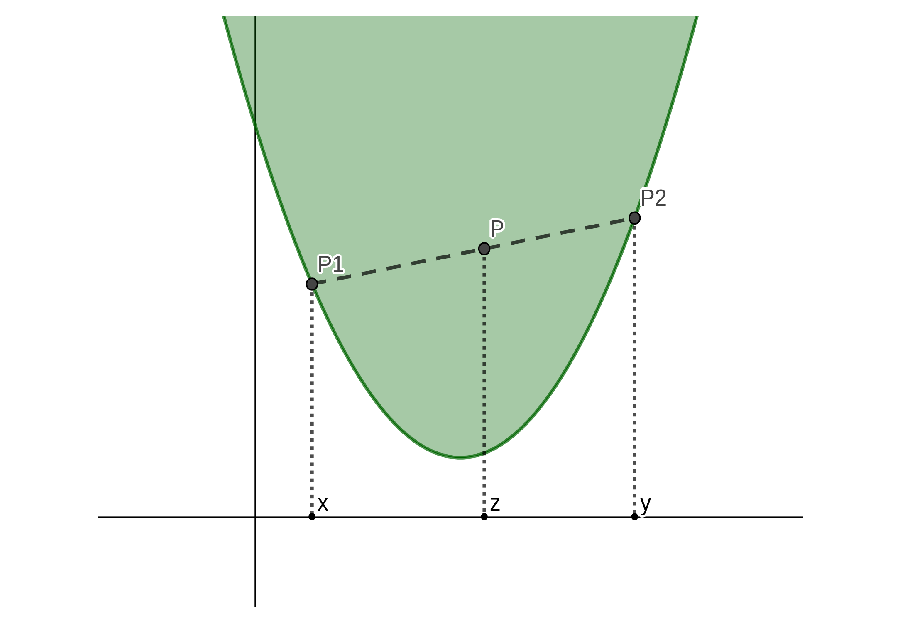
\includegraphics[scale=0.5]{convexo.eps}
	\end{center}
	\caption{Función convexa.}
	\label{fig2_1}
\end{figure}

\begin{definition}
	Un conjunto $M \subseteq V$ en un espacio vectorial real $V$ es convexo, si todas las líneas de conexión entre los puntos del conjunto están completamente en $M,$ esto es, para $x, y \in M$ se tiene $$x+\lambda(y-x) \in M \hspace{1cm} \forall \lambda \in [0,1].$$
\end{definition}
A \textit{grosso modo}, una función de una variable real es una función convexa cuando el subconjunto de $\mathbb{R}^2$ que queda por encima de la gráfica de la función es convexo. Si $z \in [x,y],$ entonces $$z = x+\lambda(y-x)\hspace{1cm}\exists \lambda \in [0,1],$$ ya que los intervalos en $\mathbb{R}$ son conjuntos convexos. Si $g$ es la recta secante formada por los puntos $P_1$ y $P_2$ de la figura \ref{fig2_1}, entonces tenemos que
\begin{align*}
	g(z) &= \frac{f(y)-f(x)}{y-x}(z-x)+f(x)\\
	&= \frac{f(y)-f(x)}{y-x}(x+\lambda(y-x)-x)+f(x)\\
	&= (1-\lambda)f(x)+\lambda f(y).
\end{align*}
Como la recta $g$ está sobre la gráfica de $f$ para todo punto de $[x,y],$ entonces $$f(z) \leq g(z) \hspace{1cm} \forall z \in [x,y].$$ Lo anterior conlleva a la siguiente definición.
\begin{definition}[Función convexa]
	Una función $f: D \rightarrow \mathbb{R}$ sobre un intervalo $D \subseteq \mathbb{R}$ es convexa si $\ \forall x, y \in D$ $$f((1-\lambda)x+\lambda y) \leq (1-\lambda)f(x)+\lambda f(y) \hspace{1cm} \forall \lambda \in [0,1].$$ 
\end{definition}
En los cursos elementales de cálculo se ha tratado la definición geométrica de convexidad para trabajar con el trazado de curvas o con problemas de optimización, usando la derivada de primer y segundo orden de la función. La siguiente proposición es útil para saber la monotonía local de una función. Su demostración es sencilla si se usa el teorema del valor medio, y la definición formal de derivada de una función sobre algún punto.
\begin{proposition}
	Sea $f:[a,b] \rightarrow \mathbb{R}$ una función continua y diferenciable en $(a,b),$ entonces $$f'(x) \geq 0 \hspace{0.5cm} \forall x \in (a,b) \hspace{0.5cm} \textrm{ssi}\hspace{0.5cm} f\  \textrm{es monótona creciente en}\ (a,b).$$
\end{proposition}
Vemos que la diferenciabilidad juega un papel clave para conocer el comportamiento de una curva, en particular, si es convexa o no en algún intervalo. La siguiente proposición determina si una función es localmente convexa.
\begin{proposition}
	Sea $f:[a,b] \rightarrow \mathbb{R}$ una función continua y dos veces diferenciable en $(a,b),$ entonces $$f''(x) \geq 0 \hspace{0.5cm} \forall x \in (a,b) \hspace{0.5cm} \textrm{ssi}\hspace{0.5cm} f\  \textrm{es convexa en}\ (a,b).$$
\end{proposition}
\begin{proof}
	Supongamos que $f''(x) \geq 0\hspace{0.2 cm} \forall x \in (a,b).$ Sean $x,y \in (a,b)$ tales que $a<x<y<b,$ entonces si consideramos la siguiente diferencia
	\begin{align*}
	(1-\lambda)f(x)+\lambda f(y)-f((1-\lambda)x+\lambda y) \hspace{2cm} \forall \lambda \in (0,1),\\
	\intertext{tenemos que, es equivalente a la expresión}
	(1-\lambda)(f(x)-f(x+\lambda (y-x)))-\lambda (f(x+\lambda (y-x))-f(y)).
	\end{align*}
	Aplicando el teorema del valor medio en los intervalos $(x,x+\lambda (y-x))$ y $(x+\lambda (y-x),y),$ obtenemos los valores intermedios $z_1, z_2 \in (a,b)$ tales que $$x<z_1<x+\lambda (y-x)<z_2<y$$
	con
	\begin{align*}
	(1-\lambda)f(x)&+\lambda f(y)-f((1-\lambda)x+\lambda y)\\
	&= (1-\lambda)f'(z_1)(x-(x+\lambda (y-x)))-\lambda f'(z_2)(x+\lambda (y-x)-y)\\
	&= (1-\lambda)\lambda (y-x)(f'(z_2)-f'(z_1)) 
	\end{align*}
	Ahora, el teorema del valor medio puede aplicarse una vez más a la función $f',$ en este caso, $\exists z_3 \in (z_1,z_2)$ tal que
	\begin{align*}
	(1-\lambda)f(x)+\lambda f(y)-&f((1-\lambda)x+\lambda y)\\
	&= (1-\lambda)\lambda (y-x)f''(z_3)(z_2-z_1).
	\end{align*}
	Por hipótesis, tenemos que $f''(z_3) \geq 0,$ así $$f((1-\lambda)x+\lambda y) \leq (1-\lambda)f(x)+\lambda f(y)\hspace{1cm}\forall \lambda \in (0,1)$$ luego, $f$ es convexa en el intervalo $(a,b).$
	Supongamos ahora que $f$ es convexa en $(a,b),$ si definimos la función $g: (0,1) \rightarrow \mathbb{R}$ como $$g(t) = f(x)+t(f(y)-f(x)),$$ tenemos que $$f(x+t(y-x)) \leq g(t) \hspace{1cm} \forall t \in (0,1).$$
	Ahora, sean $x, y \in (a,b)$ con $x<y$ y sea $$z = x+t(y-x),$$ entonces $$\frac{f(z)-f(x)}{z-x} \leq \frac{g(t)-g(0)}{t(y-x)} = \frac{f(y)-f(x)}{y-x}$$ ya que $t \neq 0.$ De manera análoga obtenemos $$\frac{f(z)-f(y)}{z-y} \geq \frac{g(1)-g(t)}{(1-t)(y-x)} = \frac{f(y)-f(x)}{y-x}$$ ya que $t \neq 1.$
	Si $z \rightarrow x,$ llegamos a $$f'(x) \leq \frac{f(y)-f(x)}{y-x},$$ igualmente con $z \rightarrow y$ $$f'(y) \geq \frac{f(y)-f(x)}{y-x}.$$ Así, $f'(x) \leq f'(y),$ lo que implica que $f'$ es monótona creciente en $(a,b).$ Luego, por proposición 2.3, $$f''(x) \geq 0 \hspace{1cm} \forall x \in (a,b).$$
\end{proof}
Por simple inspección, usando la definición de función convexa, podemos demostrar que la suma de dos funciones convexas es también una función convexa. Además, el producto de un número real con una función convexa es igualmente una función convexa. La siguiente proposición será de gran utilidad para la demostración del teorema de Bohr-Mollerup.
\begin{proposition}
	Si $f: I \rightarrow \mathbb{R}$ es convexa en el intervalo $I,$ $x_0 \in I$ y $g$ está definida como $$g(x) = \frac{f(x)-f(x_0)}{x-x_0} \hspace{1cm} \forall x \in I,\ x \neq x_0$$
	entonces, $g$ es monótona creciente.
\end{proposition}
\begin{proof}
	Sea $x_0$ un punto interior de $I$ y sean $x_1, x_2 \in I$ diferentes de $x_0$ tales que $x_1 < x_2$, entonces hay 2 casos referentes a estos puntos con respecto de $x_0$: si $x_0 < x_1$ o $x_1 < x_0,$ y además el último caso posee 2 posibilidades, $x_1 < x_2 < x_0$ o $x_1 < x_0 < x_2.$
	Si $x_1 < x_2 < x_0$ y $$t = \frac{x_0-x_2}{x_0-x_1} = \frac{x_2-x_0}{x_1-x_0},$$ claramente vemos que $0 < t < 1$ y que $x_2 = (1-t)x_0+tx_1.$
	Como $f$ es convexa, entonces $$f(x_2) \leq (1-t)f(x_0)+tf(x_1)$$ lo que implica que $$f(x_2)-f(x_0) \leq \frac{x_2-x_0}{x_1-x_0}(f(x_1)-f(x_0)),$$ además vemos que $x_2-x_0 < 0,$ entonces obtenemos que $$g(x_1) \leq g(x_2).$$
	Si $x_0 < x_1 < x_2$ y $t = \tfrac{x_1-x_0}{x_2-x_0},$ entonces $$f(x_1)-f(x_0) \leq \frac{x_1-x_0}{x_2-x_0}(f(x_2)-f(x_0))$$ y como $x_1-x_0 > 0,$ llegamos a que $$g(x_1) \leq g(x_2).$$
	Faltaría el caso $x_1 < x_0 < x_2,$ si $t = \frac{x_0-x_1}{x_2-x_1},$ entonces se tiene por convexidad de $f$ que $$f(x_0)-f(x_1) \leq \frac{f(x_2)-f(x_1)}{x_2-x_1}(x_0-x_1)$$ y como $x_2-x_1 > 0,$ esto implica que $$(f(x_0)-f(x_1))(x_2-x_1) \leq (f(x_2)-f(x_1))(x_0-x_1).$$ Pero sabemos que $$f(x_2)-f(x_1) = f(x_2)-f(x_0)-(f(x_1)-f(x_0)),$$ entonces
	\begin{align*}
	(f(x_0)-f(x_1))(x_2-x_1) &\leq \\ 
	&(f(x_2)-f(x_0))(x_0-x_1)-(f(x_1)-f(x_0))(x_0-x_1)\\
	\end{align*}
	lo que conduce a $$(f(x_0)-f(x_1))(x_2-x_0) \leq (f(x_2)-f(x_0))(x_0-x_1),$$
	y como $(x_2-x_0) > 0$ y $(x_0-x_1) > 0,$ así llegamos a $$g(x_1) \leq g(x_2).$$
	Luego, para todos los casos se cumple que si $x_0$ es un punto interior de $I,$ entonces $g$ es monótona creciente $\forall x \in I$ con $x \neq x_0.$ Por lo tanto, $x_0 \in I$ me implica que $g$ es monótona creciente $\forall x \in I$ con $x \neq x_0.$
\end{proof}
Ahora, el siguiente teorema muestra que una condición necesaria para la convexidad de una función sobre un intervalo abierto de la recta real, es que tal función sea continua sobre ese intervalo.
\begin{theorem}
	Sea $f: I \rightarrow \mathbb{R}$ convexa sobre un intervalo abierto $I,$ entonces f es continua.
\end{theorem}
\begin{proof}
	Sea $f$ convexa sobre $(a,b)$ y sean $r, s, u, v, t \in (a,b)$ tales que $$a < r < s < u < v < t < b.$$ Como $u \in (s,v),$ entonces $u = s+z(v-s)  \hspace{0.2cm} \exists z \in (0,1).$ Por convexidad de $f$ en $(a,b)$ tenemos que
	\begin{align*}
	f(u) = f(s+z(v-s)) &\leq f(s)+z(f(v)-f(s))\\
	&= f(s)+(s+z(v-s)-s)\left(\frac{f(v)-f(s)}{v-s}\right)\\
	&=f(s)+(u-s)\left(\frac{f(v)-f(s)}{v-s}\right).
	\end{align*}
	De la misma forma, para $v \in (u,t)$ obtenemos $$f(v) \leq f(u)+(v-u)\left(\frac{f(t)-f(u)}{t-u}\right),$$ y así, $$f(s)+\frac{f(u)-f(s)}{u-s}(v-s) \leq f(v) \leq f(u)+\frac{f(t)-f(u)}{t-u}(v-u).$$
	Sea $\{v_n\}_{n \in \mathbb{N}}$ una sucesión en $(u,t)$ convergente tal que $v_n \rightarrow u,$ entonces por propiedad de estricción $$\lim_{n \rightarrow \infty}\ f(v_n) = f(u),$$ lo que implica que $$\lim_{x \rightarrow u^+}\ f(x) = f(u).$$ Ahora, para $s \in (r,u)$ se tiene $$f(s) \leq f(r)+\frac{f(u)-f(r)}{u-r}(s-r),$$ que conduce a la desigualdad $$f(u)+\frac{f(v)-f(s)}{v-s}(s-u) \leq f(s) \leq f(r)+\frac{f(u)-f(r)}{u-r}(s-r).$$
	Sea $\{s_n\}_{n \in \mathbb{N}}$ una sucesión en $(r,u)$ convergente tal que $s_n \rightarrow u$ entonces, nuevamente por propiedad de estricción $$\lim_{n \rightarrow \infty}\ f(s_n) = f(u),$$ lo que conlleva a que $$\lim_{x \rightarrow u^-}\ f(x) = f(u).$$ Luego, como $u \in (a,b)$ es arbitrario, por lo tanto $f$ es continua en $(a,b).$
\end{proof}
Por último, se introduce el concepto de convexidad logarítmica o log-convexidad, el cual es de gran utilidad para el presente trabajo.
\begin{definition}
	Sea $f: I \rightarrow \mathbb{R}$ una función de valores positivos en un intervalo $I,$ entonces se dice que $f$ es log-convexa en $I$ si la función $g: I \rightarrow \mathbb{R},$ tal que $g(x) = \ln f(x),$ es convexa.
\end{definition}
\begin{proposition}
	Sea $\{f_n\}_{n \in \mathbb{N}}$ una sucesión de funciones log-convexas en un intervalo $I$ y $$\lim_{n\rightarrow\infty} f_n(x) = f(x) > 0 \hspace{1cm} \forall x \in I,$$ entonces $f$ es log-convexa en $I.$
\end{proposition}
\begin{proof}
	Sean $f_n: I \rightarrow \mathbb{R}$ funciones log-convexas y sea $$f(x) = \lim_{n \rightarrow \infty}\ f_n(x)$$ con $f(x) > 0\ \forall x \in I,$ entonces $h_n(x) = \ln f_n(x)$ son funciones convexas en $I$ $\forall n \in \mathbb{N},$ por lo cual, $\forall x, y \in I$ y $\forall \lambda \in [0,1]$ $$\ln f_n((1-\lambda)x+\lambda y) \leq (1-\lambda)\ln f_n(x)+\lambda \ln f_n(y)\hspace{0.5cm}\forall n \in \mathbb{N}.$$ Haciendo $n \rightarrow \infty$ y por continuidad de la función $\ln,$ tenemos que $$\ln f((1-\lambda)x+\lambda y) \leq (1-\lambda)\ln f(x)+\lambda\ln f(y).$$
	Por lo tanto, $f$ es log-convexa en $I.$
\end{proof}
De manera similar se puede demostrar que una sucesión de funciones convexas converge puntualmente a una función convexa, aunque no es necesario, ya que la propiedad de log-convexidad implica la convexidad de una función. El siguiente teorema muestra lo dicho anteriormente, y para su demostración es necesaria la desigualdad de Young.
\begin{lemma}[Desigualdad de Young]
	Para $a,b \in (0,\infty)$ y $p, q \in (1,\infty)$ con $\tfrac{1}{p}+\tfrac{1}{q} = 1,$ $$ab \leq \frac{1}{p}a^p+\frac{1}{q}a^q.$$
\end{lemma}
\begin{proof}
	Definimos la función $g: (0,\infty) \rightarrow \mathbb{R}$ tal que $$g(x) = x^\alpha - \alpha x\hspace{1cm} \forall \alpha \in (0,1).$$ Si generamos el polinomio de Taylor de primer grado con resto de Lagrange alrededor de $x_0 = 1,$ obtenemos $$g(x) = 1-\alpha + \tfrac{1}{2}\alpha (\alpha -1)\xi^{\alpha -2}(x-1)^2\hspace{1cm} \exists \xi \in (1,x),$$ y como $\alpha < 1,$ entonces $$g(x) \leq 1-\alpha \hspace{1cm} \forall x \in (0,\infty).$$
	Tomando $a,b \in (0,\infty)$ y $p, q \in (1,\infty)$ con $\tfrac{1}{p}+\tfrac{1}{q} = 1,$ nos conduce a que $\tfrac{1}{p}, \tfrac{1}{q} \in (0,1)$ y además, usando la anterior desigualdad con $x = \left(\tfrac{a^p}{b^q}\right),$ obtenemos
	\begin{align*}
	ab &= (a^p)^{1/p}(b^q)^{1-1/p}\\
	&= b^q\left(\frac{a^p}{b^q}\right)^{1/p}\\
	&\leq b^q\left(1-\frac{1}{p}+\frac{1}{p} \frac{a^p}{b^q}\right)\\
	&= \left(1-\frac{1}{p}\right)b^q+\frac{1}{p}a^p\\
	&= \frac{1}{p}a^p+\frac{1}{q}b^q.
	\end{align*}
\end{proof}
\begin{theorem}
	Sea $f: I \rightarrow \mathbb{R}$ una función log-convexa en $I,$ entonces $f$ es convexa en $I.$
\end{theorem}
\begin{proof}
	Sea $f: I \rightarrow \mathbb{R}$ una función log-convexa, entonces $\forall x, y \in I$ $$\ln f((1-\lambda)x+\lambda y) \leq (1-\lambda)\ln f(x)+\lambda \ln f(y)\hspace{1cm} \forall \lambda [0,1].$$ Así, por monotonía de la función exponencial, tenemos que $$f((1-\lambda)x+\lambda y) \leq f(x)^{1-\lambda}f(y)^{\lambda}\hspace{1cm} \forall \lambda \in [0,1].$$
	Como $f(x) > 0$ $\forall x \in I,$ entonces por desigualdad de Young con $p = \tfrac{1}{1-\lambda}$ y $q = \tfrac{1}{\lambda}$ se obtiene $$f((1-\lambda)x+\lambda y) \leq (1-\lambda)f(x)+\lambda f(y),$$ por lo tanto, $f$ es convexa.
\end{proof}
\section{El producto infinito de Euler}
En el capítulo anterior, partimos de la definición 1.1 de función factorial para llegar al producto infinito de Euler. En esta sección se procede de manera similar, pero en vez de usar la expresión factorial, se usa una función elemental muy conocida. Consideremos para $x > -1$ la función $$f(x) = \ln (1+x).$$ Usando el teorema de Taylor con resto de Lagrange alrededor de $x_0 = 0,$ tenemos que para $x > 0,$ $\exists c \in (0,x)$ tal que $$\ln (1+x) = x-\frac{x^2}{2(1+c)^2}.$$ Vemos que $$0 < \frac{x^2}{2(1+c)^2} = x-\ln (1+x),$$ y como $c > 0,$ entonces $$0 < \frac{x^2}{2(1+c)^2} < \frac{x^2}{2}\hspace{1cm}\forall x > 0$$ y así,
\begin{equation}
0 < x-\ln (1+x) < \frac{x^2}{2}\hspace{1cm}\forall x > 0.
\end{equation}
Reemplazando $x$ por $\tfrac{x}{k}$ en la desigualdad (2.1), donde $k \in \mathbb{N},$ obtenemos $$0 < \frac{x}{k}-\ln \left(1+\frac{x}{k}\right) < \frac{x^2}{2k^2}\hspace{1cm}\forall x > 0\hspace{0.5cm}\textrm{y}\hspace{0.5cm} \forall k \in \mathbb{N},$$ y luego $\forall n \in \mathbb{N},$ se realizan las sumas para $k \in \{1,\dots,n\}.$ Así, llegamos a
\begin{equation}
0 < \left(\sum_{k = 1}^{n}\frac{1}{k}\right)x-\ln \prod_{k = 1}^{n} \left(1+\frac{x}{k}\right) < \frac{x^2}{2}\sum_{k = 1}^{n} \frac{1}{k^2}\hspace{1cm}\forall x > 0.
\end{equation}
Si $\forall n \in \mathbb{N}$ denotamos $$P_n = \prod_{k = 1}^{n}\left(1+\frac{x}{k}\right), \hspace{1cm} u_n = \left(\sum_{k = 1}^{n}\frac{1}{k}\right)x-\ln P_n,$$ podemos escribir la desigualdad (2.2) como
\begin{equation}
0 < u_n < \frac{x^2}{2}\sum_{k = 1}^{n}\frac{1}{k^2}.
\end{equation}
Tenemos que determinar la convergencia de la sucesión $\{u_n\}_{n \in \mathbb{N}}.$ Primero, veamos si es acotada.
\begin{proposition}
	La serie infinita de términos positivos $$\sum_{k = 1}^{\infty}\frac{1}{k^2}$$ es convergente.
\end{proposition}
\begin{proof}
	Sea $\{s_n\}_{n \in \mathbb{N}}$ una sucesión de sumas parciales tales que $$s_n = \sum_{k = 1}^{n}\frac{1}{k^2}\hspace{1cm}\forall n \in \mathbb{N}.$$ Vemos que
	\begin{align*}
	s_n &= \sum_{k = 0}^{n-1}\frac{1}{(k+1)(k+1)}\\
	&< 1+\sum_{k = 1}^{n-1}\frac{1}{k(k+1)}.
	\end{align*}
	Ahora, note que la serie $$\sum_{k = 1}^{\infty}\frac{1}{k(k+1)}$$ es convergente, ya que
	\begin{align*}
	\sum_{k = 1}^{\infty}\frac{1}{k(k+1)} &= \sum_{k = 1}^{\infty}\left(\frac{1}{k}-\frac{1}{k+1}\right)\\
	&= \lim_{n \rightarrow \infty}\left(\sum_{k = 1}^{n}\frac{1}{k}-\sum_{k = 2}^{n+1}\frac{1}{k}\right)\\
	&= \lim_{n\rightarrow\infty}\left(1-\frac{1}{n+1}\right)\\
	&= 1.
	\end{align*}
	Luego, $$\sum_{k = 1}^{\infty}\frac{1}{k^2} < 1+\sum_{k = 1}^{\infty}\frac{1}{k(k+1)} = 2.$$ Así, la sucesión $\{s_n\}_{n \in \mathbb{N}}$ es monótona creciente y acotada superiormente, por lo tanto es convergente.
\end{proof}
Como consecuencia de la proposición anterior y de la desigualdad (2.3), la sucesión $\{u_n\}_{n \in \mathbb{N}}$ es una sucesión acotada para $x > 0.$ Ahora, veamos si la sucesión es monótona creciente. Para $n \in \mathbb{N}$ tenemos que
\begin{align*}
u_{n+1}-u_n &= \left(\sum_{k = 1}^{n+1}\frac{1}{k}\right)x-\ln P_{n+1}-\left(\sum_{k = 1}^{n}\frac{1}{k}\right)x+\ln P_n\\
&= \frac{x}{n+1}-\ln \frac{P_{n+1}}{P_n},\\
\intertext{y esto implica que}
u_{n+1}-u_n &= \frac{x}{n+1}-\ln \left(1+\frac{x}{n+1}\right)
\end{align*} 
donde $x > 0$ y $n \in \mathbb{N}.$
Como $\exp x \geq 1+x\hspace{0.2cm} \forall x \in \mathbb{R},$ entonces $\forall x>0$ $$\ln (1+x) < x$$ y así, $$\frac{x}{n+1}-\ln \left(1+\frac{x}{n+1}\right) > 0,$$ lo que implica que $u_{n+1}-u_n > 0,$ luego $\{u_n\}_{n \in \mathbb{N}}$ es monótona estrictamente creciente para $x > 0.$ Por lo tanto, $\{u_n\}_{n \in \mathbb{N}}$ es una sucesión convergente $\forall x > 0.$

Si sumamos y restamos $x\ln n$ a la expresión del término general de $\{u_n\}_{n \in \mathbb{N}},$ obtenemos para $n \in \mathbb{N}$
\begin{align*}
u_n &= \left(\sum_{k = 1}^{n}\frac{1}{k}\right)x-\ln P_n+x\ln n-x\ln n\\
&= \left(\sum_{k = 1}^{n}\frac{1}{k}-\ln n\right)x+\ln \frac{n^x}{P_n},
\end{align*}
y como $x > 0,$
\begin{equation}
\frac{u_n}{x} = \sum_{k = 1}^{n}\frac{1}{k}-\ln n+\frac{1}{x}\ln \frac{n^x}{P_n}.
\end{equation}
Definimos la sucesión $\{\gamma_n\}_{n \in \mathbb{N}}$ con término general $$\gamma_n = \sum_{k = 1}^{n}\frac{1}{k}-\ln n\hspace{1cm}\forall n \in \mathbb{N}.$$ Ahora, veamos si esta sucesión es convergente o no.
\begin{proposition}
	La sucesión $\{\gamma_n\}_{n \in \mathbb{N}}$ tal que $\forall n \in \mathbb{N}$ $$\gamma_n = \sum_{k = 1}^{n}\frac{1}{k}-\ln n,$$ es convergente.
\end{proposition}
\begin{proof}
	Sea $x > -1,$ y usando el teorema del valor medio para $f(x) = -\ln (1+x)+\frac{x}{1+x},$ tenemos que existe un $\xi$ entre $0$ y $x$ tal que $$-\ln (1+x)+\frac{x}{1+x} = \left(-\frac{1}{\xi+1}+\frac{1}{(\xi+1)^2}\right)x$$ con $0 < \xi < x$ o $-1 < x < \xi < 0.$ Vemos que para ambos casos $$-\ln (1+x)+\frac{x}{1+x} = \left(\frac{-\xi}{(\xi+1)^2}\right)x < 0,$$ lo que implica que $$\frac{x}{1+x}<\ln (1+x)\hspace{1cm}\forall x > -1\hspace{0.3cm} \textrm{y}\hspace{0.3cm} x \neq 0.$$
	Así, haciendo $x = \tfrac{1}{k}\hspace{0.2cm}\forall k \in \mathbb{N},$ tenemos
	\begin{equation}
	\frac{1}{k+1} = \frac{1/k}{1+1/k} < \ln \left(1+\frac{1}{k}\right) < \frac{1}{k},
	\end{equation}
	y sumando para $k \in \{1,2,\cdots,n\}$ nos conlleva a $$\sum_{k = 1}^{n}\frac{1}{k+1} < \sum_{k = 1}^{n}\ln \left(1+\frac{1}{k}\right) < \sum_{k = 1}^{n}\frac{1}{k}\hspace{1cm}\forall n \in \mathbb{N}.$$
	Como $\ln (1+1/k) = \ln(k+1)-\ln k,$ entonces
	\begin{align*}
	\sum_{k = 1}^{n}\ln \left(1+\frac{1}{k}\right) &= \sum_{k = 2}^{n+1}\ln k-\sum_{k = 1}^{n}\ln k\\
	&= \ln (n+1),
	\end{align*}
	lo que implica
	\begin{equation}
	\sum_{k = 1}^{n}\frac{1}{k+1} < \ln (n+1) < \sum_{k = 1}^{n}\frac{1}{k}\hspace{1cm}\forall n \in \mathbb{N}.
	\end{equation}
	Partiendo del siguiente resultado que involucra la parte derecha de la desigualdad (2.6) $\forall n \in \mathbb{N}$
	\begin{align*}
	0 < \ln \left(1+\frac{1}{n}\right) &= \ln (n+1)-\ln n\\
	&< \sum_{k = 1}^{n}\frac{1}{k}-\ln n\\
	&= \gamma_n,
	\end{align*}
	llegamos a que $\{\gamma_n\}_{n \in \mathbb{N}}$ está acotada inferiormente con $$0 < \ln \left(1+\frac{1}{n}\right) < \gamma_n\hspace{1cm}\forall n \in \mathbb{N}.$$
	Además, por la parte izquierda de la desigualdad (2.6) tenemos que$$\gamma_{n+1} = \sum_{k = 1}^{n+1}\frac{1}{k}-\ln (n+1) < 1$$
	y como $\gamma_1 = 1-\ln 1 = 1,$ se determina una cota superior para $\{\gamma_n\}_{n \in \mathbb{N}},$ la que conduce a $$0 < \gamma_n \leq 1\hspace{1cm}\forall n \in \mathbb{N}.$$
	Así, $\{\gamma_n\}_{n \in \mathbb{N}}$ es una sucesión acotada. Ahora, necesitamos saber si es monótona creciente o decreciente. Para $n \in \mathbb{N},$ tenemos que
	\begin{align*}
	\gamma_{n+1}-\gamma_n &= \sum_{k = 1}^{n+1}\frac{1}{k}-\ln (n+1)-\sum_{k = 1}^{n}\frac{1}{k}+\ln n\\
	&= \frac{1}{n+1}-\ln \left(1+\frac{1}{n}\right).
	\end{align*}
	Como $\frac{1}{n+1} < \ln \left(1+\frac{1}{n}\right)\hspace{0.2cm}\forall n \in \mathbb{N},$ por la parte izquierda de (2.5), entonces $$\gamma_{n+1}-\gamma_n < 0\hspace{1cm}\forall n \in \mathbb{N}.$$
	Luego, $\{\gamma_n\}_{n \in \mathbb{N}}$ es una sucesión monótona estrictamente decreciente y como además, es acotada inferiormente, por lo tanto $\{\gamma_n\}_{n \in \mathbb{N}}$ es una sucesión convergente.
\end{proof}
El límite de dicha sucesión se denota como $$\gamma = \lim_{n \rightarrow \infty}\left(\sum_{k = 1}^{n}\frac{1}{k}-\ln n	\right)$$ y se denomina como la constante de Euler-Mascheroni o número gamma. Apareció por primera vez en \textit{De Progressionibus harmonicis observationes} de Euler en 1734. Euler evaluó $\gamma$ a 16 cifras decimales y luego, Lorenzo Mascheroni (1750-1800) la evaluó a 19 cifras en sus \textit{Adnotationes ad calculum integrale Euleri} en el año 1790. El número $\gamma$ aparece en la integral exponencial, en la transformada de Laplace del $\ln,$ en los diagramas de Feynman de la Teoría Cuántica de Campos (QFT) y posee una relación con la fución zeta de Riemann. Aún no se sabe si $\gamma$ es irracional o trascendente. El matemático británico G. H. Hardy (1877-1947) ofreció su cátedra saviliana en Oxford a quien demostrara la trascendencia o irracionalidad de $\gamma.$

Volviendo a (2.4), vemos que $\forall n \in \mathbb{N}$ $$u_n-x\gamma_n = \ln \frac{n^x}{P_n}\hspace{1cm}\forall x > 0.$$ Como $\{u_n\}_{n \in \mathbb{N}}$ y $\{\gamma_n\}_{n \in \mathbb{N}}$ son sucesiones convergentes, entonces $\{\ln \frac{n^x}{P_n}\}_{n \in \mathbb{N}}$ es convergente $\forall x > 0.$ Esto implica, por continuidad de $\exp,$ que la sucesión $\{g_n(x)\}_{n \in \mathbb{N}}$ donde $$g_n(x) = \frac{n^x}{xP_n}$$ converge $\forall x > 0.$ Notemos que $\forall n \in \mathbb{N}$ y $\forall x > 0$
\begin{align*}
g_n(x) &= \frac{n^x}{x\prod_{k = 1}^{n}\left(1+\frac{x}{k}\right)}\\
&= \frac{n^x\ n!}{\prod_{k = 0}^{n}(x+k)}.
\end{align*}
Así, hemos probado que
\begin{lemma}
	Si $x > 0,$ entonces la sucesión $\{g_n(x)\}_{n \in \mathbb{N}}$ donde $g_n(x)$ está definido por
	\begin{equation}
	g_n(x) = \frac{n^x\ n!}{\prod_{k = 0}^{n}(x+k)}\hspace{2cm}\forall n \in \mathbb{N},
	\end{equation}
	es una sucesión convergente.
\end{lemma}
El límite de $g_n$ lo denominamos como producto infinito de Euler. Ahora estamos en posición de definir la función gamma a partir de dicho producto infinito.
\begin{definition}[Función gamma de Euler]
	Definimos la función $\Gamma(x)$ como
	\begin{equation}
	\Gamma(x) = \lim_{n \rightarrow \infty}\frac{n^x\ n!}{\prod_{k = 0}^{n}(x+k)}
	\end{equation}
	para todo $x$ para el cual el límite de la derecha existe y es finito. La función $\Gamma$ definida de esta manera se denomina función gamma.
\end{definition}
Sabemos por lema 2.13 que $\Gamma(x)$ está bien definida $\forall x > 0.$ El siguiente teorema caracteriza a la función gamma de Euler y determina su dominio de definición en la recta real.
\begin{theorem}
	\begin{enumerate}[(a)]
		\item La función gamma es positiva y log-convexa en el intervalo $(0,\infty).$
		\item Se cumple para la función gamma que
		\begin{equation}
		\Gamma(x+1) = x\Gamma(x)\hspace{2cm}\forall x \in Dom(\Gamma).
		\end{equation}
		\item El dominio de definición de la función gamma es $$Dom(\Gamma) = \mathbb{R}\texttt{\textbackslash}(\mathbb{Z}^-\cup \{0\}).$$
	\end{enumerate}
\end{theorem}
\begin{proof}
	\begin{enumerate}[(a)]
		\item Sabemos por (2.4) que $\forall n \in \mathbb{N}$ $$g_n(x) = \frac{n^x}{xP_n} = \frac{\exp(u_n-x\gamma_n)}{x}\hspace{1cm}\forall x > 0.$$ Denotando a $u = \lim_{n \rightarrow \infty}u_n$ y usando la definición 2.14 de función gamma $$\Gamma(x) = \frac{\exp(u-x\gamma)}{x}\hspace{1cm}\forall x > 0,$$ entonces $\Gamma(x) > 0$ $\forall x > 0.$ Siendo así, si definimos para cada $n \in \mathbb{N}$ la función $h_n$ tal que $$h_n(x) = \ln g_n(x)\hspace{1cm}\forall x > 0\,$$ tenemos por (2.7) que $\forall n \in \mathbb{N}$
		\begin{align*}
		h_n(x) &= x\ln n + \ln n! - \sum_{k = 0}^{n}\ln (x+k)\\
		&= x\ln n + \sum_{k = 0}^{n}\left[\ln (k+1)-\ln (x+k)\right].
		\end{align*}
		Vemos que $\forall x > 0,$ $h_n(x)$ es 2-veces diferenciable $\forall n \in \mathbb{N},$ lo que nos conduce a $$h_n''(x) = \sum_{k = 0}^{n}\frac{1}{(x+k)^2}\, > 0.$$ Por proposición 2.4, $g_n(x)$ es convexa en el intervalo $(0,\infty),$ $\forall n \in \mathbb{N}.$ Así, como $$\Gamma(x) = \lim_{n \rightarrow \infty}g_n(x)\hspace{1cm}\forall x \in (0,\infty)$$ y $\Gamma(x) > 0$ en dicho intervalo, por proposición 2.8 tenemos que $\Gamma$ es log-convexa en $(0,\infty).$
		\item Por definición 2.14 vemos que $\Gamma(x)$ no está definido si $x \in \mathbb{Z}^-\cup \{0\}$ y, como consecuencia, que $Dom(\Gamma) \subseteq \mathbb{R}\texttt{\textbackslash}(\mathbb{Z}^-\cup\{0\}).$
		Sea $x \in Dom(\Gamma),$ entonces $x \notin \mathbb{Z}^-\cup\{0\},$ así
		\begin{align}
			g_n(x+1) &= \frac{n^{x+1}\ n!}{\prod_{k = 0}^{n}(x+1+k)} \nonumber\\
			&= \frac{n^{x+1}\ n!}{\prod_{k = 1}^{n+1}(x+k)} \nonumber \\
			&= x\ \frac{n^x\ n!}{\prod_{k = 0}^{n}(x+k)}\cdot \frac{n}{x+n+1}.
		\end{align}
		Haciendo $n \rightarrow \infty,$ vemos que el lado derecho de (2.10) converge a $x\Gamma(x)$, y así el lado izquierdo converge también hacia el mismo límite. Luego, por definición 2.14 tenemos que $$\Gamma(x+1) = x\Gamma(x)\hspace{2cm}\forall x \in Dom(\Gamma).$$
		\item Por (b), vemos que $x \in Dom(\Gamma)$ implica que $x+1 \in Dom(\Gamma).$ Ahora, tomando $x \in Dom(\Gamma)\texttt{\textbackslash}\{1\}$ se tiene que $x \notin \mathbb{Z}^-\cup \{0,1\}$ y que el límite en (2.8) existe y es finito. Como
		\begin{equation}
		\frac{n^{x-1}\ n!}{\prod_{k = 0}^{n}(x-1+k)} = \frac{1}{x-1}\cdot\frac{n^x\ n!}{\prod_{k = 0}^{n}(x+k)}\cdot \frac{x+n}{n},
		\end{equation}
		cuando $n \rightarrow \infty,$ el lado derecho de la igualdad (2.11) converge a $\frac{\Gamma(x)}{x-1},$ y en consecuencia, el lado izquierdo también. Pero el lado izquierdo por definición 2.14 es $\Gamma(x-1),$ así $$\Gamma(x-1) = \frac{\Gamma(x)}{x-1}\hspace{1cm}\textrm{si}\hspace{0.5cm}x \in Dom(\Gamma)\texttt{\textbackslash}\{1\}$$ y que $x \in Dom(\Gamma)\texttt{\textbackslash}\{1\}$ implica que $x-1 \in Dom(\Gamma).$
		Por lema 2.13 sabemos que $(0,\infty)\subseteq Dom(\Gamma),$ entonces faltaría por probar, que para $n \in \mathbb{N}$ se tiene que $\Gamma(x)$ está definido $\forall x \in (-n,-n+1).$ Pero primero, por medio de inducción matemática probamos que $\forall n \in \mathbb{N}$
		\begin{equation}
		\Gamma(x) = \frac{\Gamma(x+n)}{\prod_{k = 0}^{n-1}(x+k)}\hspace{1cm}\forall x \in Dom(\Gamma).
		\end{equation}
		De hecho, para $n = 1$ se verifica como consecuencia de (b), ya que $$\Gamma(x) = \frac{\Gamma(x+1)}{x}\hspace{2cm}\forall x \in Dom(\Gamma).$$ Supongamos que (2.12) se cumple $\exists n \in \mathbb{N}$ (hipótesis de inducción) y como $x+n \in Dom(\Gamma),$ entonces $x+n+1 \in Dom(\Gamma),$ por consiguiente $$\Gamma(x+n+1) = (x+n)\Gamma(x+n).$$
		Usando la hipótesis de inducción llegamos a
		\begin{align*}
		\Gamma(x) &= \frac{\Gamma(x+n)}{\prod_{k = 0}^{n-1}(x+k)}\\
		&= \frac{\Gamma(x+n+1)}{\prod_{k = 0}^{n}(x+k)}\\
		\intertext{y así,}
		\Gamma(x) &= \frac{\Gamma(x+n)}{\prod_{k = 0}^{n-1}(x+k)}\hspace{1cm}\forall n \in \mathbb{N}.
		\end{align*}
		Ahora veamos si se cumple que $\Gamma(x)$ está definido para $x \in (-n,-n+1)$ $\forall n \in \mathbb{N},$ usando nuevamente inducción matemática. Tomando $n = 1$ con $x \in (-1,0)$ vemos que $0 < x+1 < 1.$ Como $(0,\infty)\subseteq Dom(\Gamma),$ entonces $x+1 \in Dom(\Gamma)\texttt{\textbackslash}\{1\},$ y por consiguiente $x \in Dom(\Gamma)$ con $$\Gamma(x) = \frac{\Gamma(x+1)}{x}.$$
		Así, nuestra afirmación es válida para $n = 1.$ Ahora, supongamos que es válida para algún $n \in \mathbb{N}.$ Si tomamos $x \in (-n-1,-n),$ entonces $-n < x+1 < -n+1.$ Por hipótesis de inducción, $x+1 \in Dom(\Gamma)$ y además
		\begin{align*}
		\Gamma(x+1) &= \frac{\Gamma(x+1+n)}{\prod_{k = 0}^{n-1}(x+1+k)}\\
		&= \frac{\Gamma(x+n+1)}{\prod_{k = 1}^{n}(x+k)}.
		\end{align*}
		Como $x+1 \in Dom(\Gamma)\texttt{\textbackslash}\{1\}$ me implica que $x \in Dom(\Gamma)$ con $\Gamma(x) = \frac{\Gamma(x+1)}{x},$ tenemos que
		\begin{align*}
		\Gamma(x) &= \frac{\Gamma(x+n+1)}{x\prod_{k = 1}^{n}(x+k)}\\
		&= \frac{\Gamma(x+n+1)}{\prod_{k = 0}^{n}(x+k)}.
		\end{align*}
		Así, se verifica para $n+1.$ Luego, $(-n,-n+1)\subseteq Dom(\Gamma)$ $\forall n \in \mathbb{N}$ y por lo tanto $$Dom(\Gamma) = \mathbb{R}\texttt{\textbackslash}(\mathbb{Z}^-\cup \{0\}).$$
	\end{enumerate}
\end{proof}
\begin{corollary}
	La función gamma es continua.
\end{corollary}
\begin{proof}
	Por teorema 2.15(a), la función gamma es log-convexa en $(0,\infty),$ entonces por teorema 2.10, es convexa en $(0,\infty).$ Así, por teorema 2.6, es continua en $(0,\infty).$
	Si $x \in (-n,-n+1)$ donde $n \in \mathbb{N},$ entonces $0 < x+n < 1.$ Así, si para cada $n \in \mathbb{N}$ definimos la función $h_n$ como $$h_n(x) = \Gamma(x+n),$$ se tiene que $h_n$ es continua en $(-n,-n+1),$ $\forall n \in \mathbb{N}.$ Luego, por (2.12), $$\Gamma(x) = \frac{\Gamma(x+n)}{\prod_{k = 0}^{n-1}(x+k)}$$ es continua en $(-n,-n+1),$ $\forall n \in \mathbb{N},$ y además en $(0,\infty),$ por lo tanto $\Gamma$ es una función continua.
\end{proof}
\begin{corollary}
	Si $n \in \mathbb{N},$ entonces $\Gamma(x)$ es positiva o negativa en el intervalo $(-n,-n+1)$ si $n$ es par o impar respectivamente.
\end{corollary}
\begin{proof}
	Sea $x \in (-n,-n+1),$ entonces $0 < x+n < 1$ y además $\Gamma(x+n) > 0.$ En el producto $\prod_{k = 0}^{n-1}(x+k)$ hay $n$ factores negativos, así si $n$ es par entonces por (2.12), $\Gamma(x) > 0.$ Si $n$ es impar, entonces $\Gamma(x) < 0.$
\end{proof}
\begin{theorem}
	Si $x \in Dom(\Gamma)$ y $n \in \mathbb{N},$ entonces $$\lim_{n \rightarrow \infty}\frac{n^x\ (n-1)!}{\Gamma(x+n)} = 1.$$
\end{theorem}
\begin{proof}
	Tenemos para $n \in \mathbb{N}$ que 
	\begin{align*}
	\frac{\Gamma(x)}{\Gamma(x+n)} &= \frac{1}{\prod_{k = 0}^{n-1}(x+k)}\\
	&= \frac{x+n}{\prod_{k = 0}^{n}(x+k)}
	\end{align*}
	entonces, $$\frac{\Gamma(x)n^x\ (n-1)!}{\Gamma(x+n)} = \frac{n^x\ n!}{\prod_{k = 0}^{n}(x+k)}\cdot \frac{x+n}{n}.$$
	Haciendo $n \rightarrow \infty$ llegamos a $$\lim_{n \rightarrow \infty}\frac{\Gamma(x)n^x\ (n-1)!}{\Gamma(x+n)} = \Gamma(x).$$
	Vemos por teorema 2.15(a) y por corolario 2.17 que $\Gamma(x) \neq 0$ $\forall x \in Dom(\Gamma),$ así $$\lim_{n \rightarrow \infty}\frac{n^x\ (n-1)!}{\Gamma(x+n)} = 1.$$
\end{proof}
\begin{corollary}
	Sea $\Gamma$ la función gamma, entonces $$\lim_{x \rightarrow \infty}\Gamma(x) = \infty.$$
\end{corollary}
\begin{proof}
	Por teorema 2.18 sabemos que $$\lim_{n \rightarrow \infty}\frac{n^x\ (n-1)!}{\Gamma(x+n)} = 1.$$ Tomando $y > 0,$ $\exists N_1 \in \mathbb{N}$ tal que $\forall n \geq N_1$ $$-\frac{1}{2} < \frac{n^y\ \Gamma(n)}{\Gamma(y+n)}-1 < \frac{1}{2}$$ lo que implica que $$\frac{2}{3}n^y\ \Gamma(n) < \Gamma(y+n)\hspace{1cm}\forall n \geq N_1.$$
	Sea $N = max\{N_1,2\},$ tomando a $x > N$ se cumple que $$\frac{2}{3}N^{x-N} \leq \frac{2}{3}N^{x-N}\Gamma(N) < \Gamma(x)$$ y así, $$\frac{2}{3}N^{x-N} < \Gamma(x)\hspace{1cm}\forall x > N \geq 2.$$
	Como $\lim_{x \rightarrow \infty}N^{x-N} = \infty\hspace{0.3cm}\forall N > 1,$ entonces $$\lim_{x \rightarrow \infty}\Gamma(x) = \infty.$$
\end{proof}
Como $\forall n \in \mathbb{N}$
\begin{align*}
\Gamma(x) &= \frac{\Gamma(x+n)}{\prod_{k = 0}^{n-1}(x+k)}\\
&= \frac{1}{x}\frac{\Gamma(x+n)}{\prod_{k = 1}^{n-1}(x+k)},
\end{align*}
por corolario 2.19, llegamos a los siguientes resultados: 
Si $x \rightarrow 0^+,$ entonces $\Gamma(x) \rightarrow \infty.$ De manera similar $$\lim_{x \rightarrow 0^-}\Gamma(x) = -\infty.$$
Además, para $n \in \mathbb{N}$ $$\lim_{x \rightarrow (-n+1)^-}\Gamma(x) = \lim_{x \rightarrow -n^+}\Gamma(x) = -\infty$$ con $n$ impar y, $$\lim_{x \rightarrow (-n+1)^-}\Gamma(x) = \lim_{x \rightarrow -n^+}\Gamma(x) = \infty$$ con $n$ par. Podemos observar claramente este comportamiento en las asíntotas verticales de la figura \ref{fig1_5}.

La fórmula de recurrencia (2.9) se denomina ecuación funcional para la función gamma de Euler. Esta ecuación no determina una única función, ya que existen diversas funciones que la cumplen (en el capítulo 1 se da un ejemplo de una función que satisface esta ecuación). El teorema de Bohr-Mollerup afirma que existe una única función $f$ que satisface la ecuación (2.9) si cumple con que: $f(1) = 1,$ y que sea positiva y logarítmicamente convexa para $x > 0.$ La existencia de una función con tales propiedades (la función gamma) se da por el teorema 2.15.
\begin{theorem}[Teorema de Bohr-Mollerup]
	Si $f$ es positiva y log-convexa para $x > 0,$ $f(1) = 1$ y que también satisface
	\begin{equation}
	f(x+1) = x f(x),
	\end{equation}
	entonces $f(x) = \Gamma(x)\ \forall x > 0.$
\end{theorem}
\begin{proof}
	Sea $f$ una función positiva y log-covexa para $x > 0,$ que $f(1) = 1$ y que satisface la ecuación (2.13). Realizando inducción matemática en $n$ con (2.13), es fácil mostrar que si $n \in \mathbb{N}$ entonces
	\begin{equation}
	f(n) = (n-1)!
	\end{equation}
	Además, para $x > 0$
	\begin{equation}
	f(x) = \frac{f(x+n)}{\prod_{k = 0}^{n-1}(x+k)}
	\end{equation}
	es cierta para $n \in \mathbb{N}.$
	
	De hecho, si $n = 1$ se verifica (2.15) $\forall x > 0$ gracias a (2.13), ya que $$f(x) = \frac{f(x+1)}{x}.$$ Supongamos que $\forall x > 0$ (2.15) se cumple $\exists n \in \mathbb{N},$ así, como $x+1 > 0$
	\begin{align*}
	f(x+1) &= \frac{f(x+1+n)}{\prod_{k = 0}^{n-1}(x+1+k)}\\
	&= \frac{f(x+n+1)}{\prod_{k = 1}^{n}(x+k)},\\
	\intertext{y por (2.13) vemos que}
	f(x) &= \frac{f(x+n+1)}{x\prod_{k = 1}^{n}(x+k)}\\
	&= \frac{f(x+n+1)}{\prod_{k = 0}^{n}(x+k)}
	\end{align*}
	lo que implica que $\forall x > 0$ (2.15) se cumple $\forall n \in \mathbb{N}.$
	Ahora, sea $x \in \left(0,1\right]$ y $n \geq 2,$ entonces
	\begin{equation}
	n-1 < n < x+n \leq n+1.
	\end{equation}
	Considere la función $g$ definida como $$g(x) = \frac{\ln f(x)-\ln f(n)}{x-n}\hspace{1cm}\forall x > 0\ \textrm{con}\ x \neq n.$$
	Como $f$ es log-convexa para $x > 0,$ es decir, $\ln f$ es convexa en $(0,\infty),$ entonces $g$ es monótona creciente por proposición 2.5. Así, lo anteriormente dicho y (2.16) implican que para $x \in \left(0,1\right]$ tenemos que
	\begin{align*}
	\frac{\ln f(n-1)-\ln f(n)}{-1} &\leq \frac{\ln f(x+n)-\ln f(n)}{x}\\
	&\leq \frac{\ln f(n+1)-\ln f(n)}{1}.
	\end{align*}
	Usando (2.14) llegamos a
	\begin{align*}
	x(\ln (n-1)!-\ln (n-2)!) &\leq \ln f(x+n)-\ln (n-1)!\\
	&\leq x(\ln n!-\ln (n-1)!)
	\end{align*}
	y por medio del uso de propiedades de las funciones $\ln$ y factorial $$x\ln (n-1)+\ln (n-1)! \leq \ln f(x+n) \leq x\ln n + \ln (n-1)!$$
	Lo anterior es equivalente a $$\ln \left[(n-1)^x\ (n-1)!\right] \leq \ln f(x+n) \leq \ln \left[n^x\ (n-1)!\right]$$ y como $\exp$ es monótona creciente $$(n-1)^x\ (n-1)! \leq f(x+n) \leq n^x\ (n-1)!$$
	Usando (2.15) nos conduce a
	\begin{equation}
	\frac{(n-1)^x\ (n-1)!}{\prod_{k = 0}^{n-1}(x+k)} \leq f(x) \leq \frac{n^x\ (n-1)!}{\prod_{k = 0}^{n-1}(x+k)}
	\end{equation}
	donde $n \geq 2$ y $x \in \left(0,1\right].$ Vemos que la desigualdad de la izquierda de (2.17) es válida $\forall n \in \mathbb{N}$ tal que $n-1 \geq 1,$ y así, después de reemplazar $n-1$ por $n,$ llegamos a $$\frac{n^x\ n!}{\prod_{k = 0}^{n}(x+k)} \leq f(x)\hspace{1cm}\textrm{para}\ n \geq 1,\ 0 < x \leq 1.$$
	Lo anterior y la desigualdad en la derecha de (2.17) implican que $$\frac{n^x\ n!}{\prod_{k = 0}^{n}(x+k)} \leq f(x) \leq \frac{n^x\ n!}{\prod_{k = 0}^{n}(x+k)}\cdot \frac{x+n}{n}$$ para $n \geq 1,$ $0 < x \leq 1.$ Haciendo $n \rightarrow \infty,$ se tiene por teorema de estricción que
	\begin{align*}
	f(x) &= \lim_{n \rightarrow \infty}\frac{n^x\ n!}{\prod_{k = 0}^{n}(x+k)}\\
	&= \Gamma(x)\hspace{3cm}\ \textrm{para}\ 0 < x \leq 1.
	\end{align*}
	Partiendo de (2.13) vemos que por inducción matemática, fácilmente obtenemos el siguiente resultado:
	\begin{equation}
	f(x+n) = \Gamma(x+n)\hspace{1.5cm}\forall x \in \left(0,1\right]\ \textrm{y}\ \forall n \in \mathbb{N}.
	\end{equation}
	Haciendo $x = 1,$ tenemos que $f$ y $\Gamma$ tienen los mismos valores para todos los números naturales, $$f(n) = \Gamma(n)\hspace{1cm}\forall n \in \mathbb{N}.$$
	Tomando $x > 1,$ donde $x \neq \mathbb{N},$ $\exists n \in \mathbb{N}$ tal que $n < x < n+1$ ($n = [x]$ con $x \neq n$), lo que implica que $0 < x-n < 1.$ Sea $y = x-n,$ entonces $0 < y < 1.$ Por (2.18) vemos que $\forall x > 1$ con $x \neq n$
	\begin{align*}
	f(x) &= f(y+n)\\
	&= \Gamma(y+n)\\
	&= \Gamma(x).\\
	\intertext{Por lo tanto,}
	f(x) &= \Gamma(x)\hspace{1cm}\ \forall x > 0.
	\end{align*}
\end{proof}
\begin{corollary}
	Sea $f$ una función definida en el conjunto $S = \mathbb{R}\texttt{\textbackslash}(\mathbb{Z}^-\cup \{0\})$ y log-convexa en $(0,\infty),$ donde $f(1) = 1$ y $f(x+1) = xf(x)$ para cada $x \in S,$ entonces $f(x) = \Gamma(x)$ para todo $x \in S.$
\end{corollary}
\begin{proof}
	Debemos probar para cada $n \in \mathbb{N}$ que $f(x) = \Gamma(x)$ $\forall x \in (-n,-n+1).$ Supongamos que $f$ cumple las condiciones descritas en la hipótesis por lo que realizamos inducción sobre $n.$ Si $n = 1,$ tomamos $x \in (-1,0)$ entonces $0 < x+1 < 1.$ Por teorema de Bohr-Mollerup $$f(x+1) = \Gamma(x+1)$$ y además, por (2.13) obtenemos
	\begin{align*}
	f(x) &= \frac{\Gamma(x+1)}{x}\\
	&= \Gamma(x)
	\end{align*}
	para $x \in (-1,0).$ Ahora, supongamos que nuestra afirmación es cierta para algún $n \in \mathbb{N}.$ Tomando a $x \in (-n-1,-n)$ nos conduce a $$-n < x+1 < -n+1,$$ por hipótesis de inducción tenemos que
	\begin{align*}
	f(x+1) &= \Gamma(x+1)\\
	\intertext{así,}
	f(x) &= \frac{\Gamma(x+1)}{x}\\
	&= \Gamma(x)
	\end{align*}
	para $x \in (-n-1,-n).$ Luego, $f(x) = \Gamma(x)$ en $(-n,-n+1)$ $\forall n \in \mathbb{N}$ y $\forall x > 0$ por teorema de Bohr-Mollerup, por lo tanto $$f(x) = \Gamma(x)\hspace{2cm}\forall x \in S.$$
\end{proof}

\section{Integral de Euler de segunda especie}
En la sección anterior partimos de la función logaritmo natural para llegar a el producto infinito de Euler, el cual es una de las 3 representaciones más distintivas de la función gamma de Euler. En los cursos de cálculo o análisis elemental, cuando nos mencionan la función gamma de Euler, esta se ve representada como una integral impropia. En esta sección llegaremos a representar la función gamma por medio de la integral de Euler de segunda especie y para ello, se hará uso de la integración de Lebesgue, la cual se encuentra explicada de manera muy detallada en los textos de Apostol (1974) y Arens (2013).

Veamos que para $\alpha > 0$ se tiene que $$\int_{0}^{\infty}\ e^{-\alpha x}\ dx = \frac{1}{\alpha},$$ y si derivamos con respecto a $\alpha$ en ambos lados (suponiendo que es permitido hacerlo) obtenemos por inducción matemática sobre $n$ que $$\int_{0}^{\infty}\ x^n\ e^{-\alpha x}\ dx = \frac{n!}{\alpha^{n+1}}\hspace{1cm}\forall n \in \mathbb{Z}_0^+.$$ Haciendo $\alpha = 1,$ llegamos a que 
\begin{equation}
	\int_{0}^{\infty}\ x^n\ e^{-x}\ dx = n!\hspace{1cm}\forall n \in \mathbb{Z}_0^+,
\end{equation}
lo que nos da una idea de representar a la función factorial por medio de una integral impropia bajo el parámetro $n$.

El procedimiento de derivación con respecto a $\alpha$ está justificado por el teorema 2.30. Los 2 teoremas siguientes son muy necesarios para el tratamiento de la integral de Euler y son los más representativos en la teoría de integración de Lebesgue.
\begin{theorem}[Teorema de Beppo Levi]
	Sea $\{f_n\}_{n \in \mathbb{N}}$ una sucesión de funciones Lebesgue-integrables en el intervalo $I,$ $f_n \in L(I)\ \forall n \in \mathbb{N},$ monótonas c.t.p. (en casi todas partes) y sea la sucesión de integrales $$\left\{\int_{I}\ f_n\ dx\right\}_{n \in \mathbb{N}}$$ acotada en $\mathbb{R}$, entonces la sucesión $\{f_n\}_{n \in \mathbb{N}}$ converge puntualmente c.t.p. a la función $f \in L(I)$ con $$\lim_{j \rightarrow \infty}\int_{I}\ f_j\ dx = \int_{I}\ f\ dx.$$
\end{theorem}
\begin{theorem}[Teorema de convergencia dominada de Lebesgue]
	Sea $\{f_n\}_{n \in \mathbb{N}}$ una sucesión de funciones Lebesgue-integrables sobre el intervalo $I,$ $f_n \in L(I)\ \forall n \in \mathbb{N},$ tales que converjan puntualmente a $f: I \rightarrow \mathbb{R}$ c.t.p., y si existe una función integrable en $I \subseteq \mathbb{R},$ $g \in L(I),$ tal que $|f_n(x)| \leq g(x)\ \forall x \in I$ c.t.p. y $\forall n \in \mathbb{N},$ entonces $f \in L(I)$ y además $$\lim_{n \rightarrow \infty}\int_{I}\ f_n(x)\ dx = \int_{I}\ f(x)\ dx.$$
\end{theorem}
Existen funciones con características particulares que nos permiten saber si la función es Lebesgue-integrable o no. Tales funciones son las denominadas funciones regladas.
\begin{definition}
	Una función $f: [a,b] \rightarrow \mathbb{R}$ es reglada si en cada punto $x_0 \in (a,b)$ existen los límites por izquierda y derecha, $\lim_{x \rightarrow x_0^-}\ f(x)$ y $\lim_{x \rightarrow x_0^+}\ f(x),$ y además, los límites $$\lim_{x \rightarrow a^+}\ f(x)\hspace{0.4cm}y\hspace{0.4cm}\lim_{x \rightarrow b^-}\ f(x)$$ existen también. 
\end{definition}
El siguiente teorema nos permite caracterizar a las funciones regladas y relacionarlas con las funciones Lebesgue-integrables.
\begin{theorem}
	Una función $f: [a,b] \rightarrow \mathbb{R}$ es reglada si y solo si existe una sucesión de funciones escalonadas $\{\phi_n \}_{n \in \mathbb{N}}$ con $\phi_n: [a,b] \rightarrow \mathbb{R}\hspace{0.3cm}\forall n \in \mathbb{N}$ tal que convergen uniformemente a $f.$
\end{theorem}
\begin{proposition}
	Toda función $f: [a,b] \rightarrow \mathbb{R}$ reglada es Lebesgue-integrable.
\end{proposition}
\begin{proof}
	Sea $f: [a,b] \rightarrow \mathbb{R}$ una función reglada, entonces existe una sucesión de funciones escalonadas $\{\phi_n\}_{n \in \mathbb{N}}$ que convergen uniformemente a $f.$ Así, existe un $N \in \mathbb{N}$ tal que $$\|f-\phi_N\|_\infty \leq 1.$$ La función escalonada $\phi_N$ toma un número finito de valores, e incluso los valores aislados en el número finito de puntos de salto. Por lo anterior, $\phi_N$ es una función acotada y esto nos conduce a $$\|f\|_\infty = \|f-\phi_N+\phi_N\|_\infty \leq 1+\|\phi_N\|_\infty.$$ Como consecuencia de la convergencia uniforme de la sucesión a $f,$ tal sucesión converge puntualmente a $f.$ Luego, por la desigualdad anterior, $f$ es acotada en el intervalo $[a,b]$ y por consiguiente está dominada por una función constante en tal intervalo. Por lo tanto, por el teorema de convergencia dominada de Lebesgue, la función límite $f$ es Lebesgue-integrable en $[a,b],$ $f \in L([a,b]).$
\end{proof}
La siguiente proposición nos permite examinar la convergencia de integrales impropias, si miramos dentro del contexto de la integración de Riemann, la cual nos permite saber si la integral de Euler está bien definida.
\begin{proposition}[Criterio de convergencia para integrales]
	Una función $f: I \rightarrow \mathbb{R}$ es Lebesgue-integrable sobre un intervalo abierto $I,$ $f \in L(I),$ si $f$ es integrable en una sucesión de subintervalos encajados $I_1 \subseteq I_2 \subseteq \dots \subseteq I \subseteq \mathbb{R}$ con $I = \bigcup_{j = 1}^\infty I_j,$ $f \in L(I_j)\ \forall j \in \mathbb{N},$ y la sucesión de integrales $$\left\{\int_{I_j}\ |f(x)|\ dx\right\}_{j \in \mathbb{N}}$$ es acotada. En ese caso, $$\int_{I}\ f(x)\ dx = \lim_{j \rightarrow \infty}\int_{I_j}\ f(x)\ dx.$$
\end{proposition}
\begin{proof}
	Sea $f: I \rightarrow \mathbb{R}$ tal que $f \geq 0$ en $I$ y sea
	\[
	f_j(x) = \left\{ \begin{array}{lcl}
	f(x),  & x \in I_j\\
	0,  & \mbox{en otro caso}
	\end{array}
	\right.
	\] para una sucesión de subintervalos encajados de $I.$ La sucesión $\{f_j\}_{j \in \mathbb{N}}$ converge puntualmente y monótonamente creciente a $f.$ Como $$\int_{I}\ f_j\ dx = \int_{I_j}\ f\ dx\hspace{0.6cm}\forall j \in \mathbb{N},$$ las sucesiones $$\left\{\int_{I}\ f_j\ dx\right\}_{j \in \mathbb{N}} = \left\{\int_{I_j}\ f\ dx\right\}_{j \in \mathbb{N}},$$ y ya que tal sucesión de integrales es acotada (por hipótesis), por teorema de Beppo Levi (teorema 2.22) tenemos que $f \in L(I)$ con $$\int_{I}\ f\ dx = \lim_{j \rightarrow \infty}\int_{I_j}\ f\ dx.$$
	Ahora, si $f: I \rightarrow \mathbb{R}$ es arbitraria, entonces descomponemos $f = f^+ - f^-$ con \[
	f^+(x) = \left\{ \begin{array}{lcl}
	f(x)  & \mbox{si } & f(x) \geq 0\\
	0  & \mbox{si} & f(x) < 0
	\end{array}
	\right.
	\] y \[
	f^-(x) = \left\{ \begin{array}{lcl}
	0  & \mbox{si } & f(x) \geq 0\\
	-f(x)  & \mbox{si} & f(x) < 0.
	\end{array}
	\right.
	\]
	Aplicando el resultado anterior para las funciones positivas, tenemos que $f \in L(I)$ con $$\int_{I}\ f\ dx = \lim_{j \rightarrow \infty}\int_{I_j}\ f\ dx.$$
\end{proof}
Gracias a la proposición 2.27, podemos determinar un criterio para la convergencia de series numéricas.
\begin{proposition}[Criterio integral para series]
	Si $f:[N,\infty] \rightarrow \mathbb{R}$ es una función monótona decreciente, positiva y Lebesgue-integrable sobre cada subintervalo compacto y sea $a_n = f(n)\ \forall n \geq N\ \exists N \in \mathbb{N},$ entonces la serie $$\sum_{n = N}^{\infty}a_n\hspace{0.3cm}\textrm{converge si y solo si}\hspace{0.3cm}\int_{N}^{\infty}f(x)\ dx\ \textrm{existe.}$$
\end{proposition}
\begin{proof}
	Como $0 \leq a_{j+1} = f(j+1) \leq f(x) \leq f(j) = a_j\ \forall j \geq N$ y $\forall x \in [j,j+1]$ y además $I_n = [N,n]\ \forall n \in \mathbb{N},$ entonces tenemos que $$\sum_{j = N+1}^{n+1}a_j \leq \int_{I_n}f(x)\ dx \leq \sum_{j = N}^{n}a_j.$$ Supongamos que $\sum_{j = N}^{\infty}a_j$ es convergente. Como $f$ es integrable en $I_n\ \forall n \in \mathbb{N}$ y la sucesión $\left\{\int_{I_n}f(x)\ dx\right\}_{n \in \mathbb{N}}$ es acotada, por teorema 2.27 tenemos que $$\int_{N}^{\infty}f(x)\ dx\hspace{0.3cm}\textrm{existe.}$$
	Por otro lado, si $\int_{N}^{\infty}f(x)\ dx$ existe, entonces la sucesión monótona decreciente $\left\{\sum_{j = N+1}^{n+1}a_j\right\}_{n \in \mathbb{N}}$ posee una cota superior, así $$\sum_{n = N}^{\infty}a_n\hspace{0.3cm}\textrm{converge.}$$
\end{proof}
La integral impropia (2.19) es un ejemplo claro de integral paramétrica, los siguientes teoremas son de gran utilidad para poder caracterizar esta integral y definir sus propiedades.
\begin{theorem}[Continuidad de las integrales paramétricas]
	Sea $f:[a,b]\times I \rightarrow \mathbb{R}$ una función tal que $f(\cdot,x)$ es continua en $[a,b]\ \forall x \in I$ c.t.p., y que además existe una función $g \in L(I)\ \forall t \in [a,b]$ tal que $$|f(t,x)| \leq g(x)\hspace{0.6cm}\forall x \in I\ \textrm{c.t.p.}$$ entonces $$G(t) = \int_{I}\ f(t,x)\ dx\hspace{0.4cm}\textrm{con}\ t \in [a,b]$$ define una función $G:[a,b] \rightarrow \mathbb{R}$ continua. 
\end{theorem}
\begin{theorem}[Derivada bajo el signo integral]
	Sea $f(\cdot,x)$ una función diferenciable en $[a,b]\ \forall x \in I$ c.t.p. con derivada $\frac{\partial f(\cdot,x)}{\partial t} = (f(\cdot,x))'$ y que además existe una función $g \in L(I)\ \forall t \in [a,b]$ con $\left|\frac{\partial f(t,x)}{\partial t}\right| \leq g(x)\ \forall x \in I$ c.t.p., entonces la integral paramétrica es diferenciable y $$G'(t) = \int_{I}\ \frac{\partial f}{\partial t}(t,x)\ dx,\hspace{0.3cm}\forall t \in [a,b].$$
\end{theorem}
Vemos que la función factorial la podemos expresar con la integral impropia (2.19) bajo el parámetro $n.$ Si extendemos el dominio de este parámetro a todos los reales $\mathbb{R}$ llegamos a la función 
\begin{equation}
	G(\alpha) = \int_{0}^{\infty}\ t^{\alpha - 1}e^{-t}\ dt.
\end{equation}
Si $\alpha - 1 < 0,$ existe una singularidad del integrando en el límite inferior $0.$ Podemos reescribir la integral como \[G(\alpha) = \overbrace{\int_{0}^{1}\ t^{\alpha - 1}e^{-t}\ dt}^{I_1} + \underbrace{\int_{0}^{\infty}\ t^{\alpha - 1}e^{-t}\ dt}_{I_2}\] para encontrar el dominio de definición de la función $G.$ Para eso, haremos uso de la siguiente proposición.
\begin{proposition}
	Sea $\alpha \in \mathbb{R},$ entonces $$\lim_{x \rightarrow \infty} \frac{x^\alpha}{e^x} = 0.$$ 
\end{proposition}
\begin{proof}
	Sea $\alpha \in \mathbb{R},$ por propiedad arquimediana $\exists n \in \mathbb{N}$ tal que $n > \alpha,$ además $$e^x > \frac{x^{n+1}}{(n+1)!}\hspace{0.4cm}\forall x > 0.$$ Si $x \geq 1,$ entonces $$\frac{e^x}{x^\alpha} \geq \frac{e^x}{x^n} > \frac{x}{(n+1)!}.$$
	Sea $M > 0,$ si $N = \max \{1, (n+1)!\ M\},$ entonces $$\frac{e^x}{x^\alpha} > M\hspace{0.3cm}\textrm{siempre que}\hspace{0.3cm}x > N,$$ así $$\lim_{x \rightarrow \infty}\frac{e^x}{x^\alpha} = \infty.$$ Por lo tanto, $$\lim_{x \rightarrow \infty} \frac{x^\alpha}{e^x} = 0.$$
\end{proof}
En la integral $I_2$ vemos que $\forall \alpha \in \mathbb{R}$ $$\lim_{t \rightarrow \infty}\frac{t^{\alpha - 1}e^{-t}}{t^{-2}} = \lim_{t \rightarrow \infty}\frac{t^{\alpha + 1}}{e^t} = 0,$$ lo que implica que $\exists M > 0$ tal que $\forall t \geq 1$ $$t^{\alpha - 1}e^{-t} \leq Mt^{-2}.$$ Donde $$\int_{1}^{b}t^{\alpha - 1}e^{-t}\ dt \leq M\int_{1}^{b}\frac{1}{t^2}\ dt = M(1- 1/b),$$ así $$\int_{1}^{\infty}t^{\alpha - 1}e^{-t}\ dt \leq M$$ por consiguiente $I_2$ está definido $\forall \alpha \in \mathbb{R}.$

Ahora para $I_1,$ vemos que presenta una singularidad en $0$ cuando $\alpha - 1 < 0.$ Como $e^{-t} \leq 1\ \forall t \geq 0,$ entonces $$t^{\alpha - 1}e^{-t} \leq t^{\alpha - 1}\hspace{0.3cm}\forall t \geq 0.$$ Así,
\begin{align*}
	\int_{a}^{1}t^{\alpha - 1}e^{-t}\ dt &\leq \int_{a}^{1}t^{\alpha - 1}\ dt \\
	&= \int_{a}^{1}t^{-(1-\alpha)}\ dt\\
	&= \left\{
	\begin{array}{lcl}
	\frac{1}{\alpha}(1-a^{\alpha})\hspace{0.3cm}&\mbox{si }\alpha \neq 0\\
	-\ln a &\mbox{si }\alpha = 0
	\end{array}
	\right.
\end{align*}
Vemos que solo para $\alpha > 0$ el límite $$\lim_{a \rightarrow 0^+}\int_{a}^{1}t^{-(1-\alpha)}\ dt$$ existe y es igual $1/\alpha$, por consiguiente $I_1$ solo está definida para $\mathbb{R}_{>0}.$ Luego, por $I_1$ y $I_2,$ la función $G$ está acotada por $$G(\alpha) \leq \frac{1}{\alpha}+M$$ y por lo tanto, por criterio de convergencia para integrales (proposición 2.27), la integral (2.20) existe solo si $\alpha > 0.$

Así llegamos a la integral de segunda especie de Euler, 
\begin{equation}
	G(x) = \int_{0}^{\infty}t^{x-1}e^{-t}\ dt\hspace{0.3cm}\textrm{para}\hspace{0.3cm}x > 0.
\end{equation}
Como $t^{x-1}e^{-t}$ es continua $\forall x \in (0,\infty)$ con $t \geq 0$ fijo en casi todas partes. Además, para cada subintervalo $[a,b]$ con $0 < a < b,$ el integrando está dominado por la función \[
g(t) = \left\{
\begin{array}{lcl}
	t^{a-1}\hspace{0.4cm} &0 < t \leq 1\\
	Mt^{-2}  &t > 1
\end{array}
\right.\]
para algún $M > 0.$ Vemos que la función $g$ es reglada y por consiguiente, Lebesgue-integrable, así $\forall x > 0$ $$t^{x-1}e^{-t} \leq g(t)\hspace{0.3cm}\forall t \in [0,\infty)\ \textrm{c.t.p.}$$ Luego por teorema 2.29, $G(x)$ es continua en $[a,b]\ $ $\forall a,b \in \mathbb{R}$ tal que $0 < a < b.$ Por lo tanto, $$G(x) = \int_{0}^{\infty}t^{x-1}e^{-t}\ dt\hspace{0.2cm}\textrm{es continua en }\ (0,\infty).$$

Veamos si la función $G$ cumple la fórmula de recurrencia (2.9). Sea $x > 0,$ por medio de integración por partes tenemos que $$G(x+1) = -t^xe^{-t}\bigg|_a^b + x\int_{a}^{b}t^{x-1}e^{-t}\ dt.$$ Si $a \rightarrow 0^+$ y $b \rightarrow \infty,$ tenemos que por proposición 2.31, 
\begin{align*}
	G(x+1) &= x\int_{0}^{\infty}t^{x-1}e^{-t}\ dt\\
	&= x\ G(x).
\end{align*}
Además $$G(1) = \int_{0}^{\infty}e^{-t}\ dt = 1-\lim_{t \rightarrow \infty}e^{-t} = 1,$$ y por medio de inducción matemática llegamos a que $G(n+1) = n!.$

La siguiente proposición es necesaria para determinar si la integral de segunda especie de Euler es logarítmicamente convexa.
\begin{proposition}[Desigualdad de Hölder para integrales]
	Sean $f,g: \mathbb{R} \rightarrow \mathbb{C}$ integrables sobre $A \subseteq \mathbb{R}$ compacto, entonces se cumple $$\int_{A}\ |f(x)||g(x)|\ dx \leq \bigg(\int_{A}\ |f(x)|^p\ dx \bigg)^{1/p}\bigg(\int_{A}\ |g(x)|^q\ dx\bigg)^{1/q}.$$
\end{proposition}
\begin{proof}
	Sean $f,g: \mathbb{R} \rightarrow \mathbb{C}$ integrables sobre $A \subseteq \mathbb{R}$ compacto, entonces por desigualdad de Young (lema 2.9) tenemos que $$\frac{|f(x)|}{\big(\int_{A}\ |f(x)|^p\ dx\big)^{1/p}}\cdot \frac{|g(x)|}{\big(\int_{A}\ |g(x)|^q\ dx\big)^{1/q}} \leq \frac{1}{p}\frac{|f(x)|^p}{\int_{A}\ |f(x)|^p\ dx}+\frac{1}{q}\frac{|g(x)|^q}{\int_{A}\ |g(x)|^q\ dx}.$$
	Integrando con respecto a $x$ en $A$ tenemos $$\frac{\int_{A}\ |f(x)||g(x)|\ dx}{\big(\int_{A}\ |f(x)|^p\ dx\big)^{1/p}\big(\int_{A}\ |g(x)|^q\ dx\big)^{1/q}} \leq \frac{1}{p}+\frac{1}{q} = 1,$$ entonces $$\int_{A}\ |f(x)||g(x)|\ dx \leq \bigg(\int_{A}\ |f(x)|^p\ dx\bigg)^{1/p}\bigg(\int_{A}\ |g(x)|^q\ dx\bigg)^{1/q}.$$
\end{proof}
Ahora, veamos si la integral $G(x)$ es una función log-convexa. Sean $x,y \in \mathbb{R}_{>0}$ y $\lambda \in (0,1).$ Si denotamos a $p = 1/\lambda$ y a $q = 1/(1-\lambda),$ entonces $p,q \in (0,\infty)$ y $\frac{1}{p}+\frac{1}{q} = 1.$ Así, 
\begin{align*}
	G(\lambda x + (1-\lambda)y) &= \int_{0}^{\infty}t^{\lambda x+(1-\lambda)y-1}e^{-t}\ dt\\
	&= \int_{0}^{\infty}t^{\frac{x}{p}+\frac{y}{q}-(\frac{1}{p}+\frac{1}{q})}e^{-t(\frac{1}{p}+\frac{1}{q})}\ dt\\
	&= \int_{0}^{\infty}(t^{x-1}e^{-t})^{1/p}(t^{y-1}e^{-t})^{1/q}\ dt\\
	&= \lim_{a \rightarrow 0^+}\lim_{b \rightarrow \infty}\int_{a}^{b}(t^{x-1}e^{-t})^{1/p}(t^{y-1}e^{-t})^{1/q}\ dt.
\end{align*}
Utilizando la desigualdad de Hölder (proposición 2.32) tenemos que 
\begin{align*}
	\int_{a}^{b}(t^{x-1}e^{-t})^{1/p}(t^{y-1}e^{-t})^{1/q}\ dt &\leq \bigg(\int_{a}^{b}t^{x-1}e^{-t}\ dt\bigg)^{1/p}\bigg(\int_{a}^{b}t^{y-1}e^{-t}\ dt\bigg)^{1/q}\\
	&= \bigg(\int_{a}^{b}t^{x-1}e^{-t}\ dt\bigg)^{\lambda}\bigg(\int_{a}^{b}t^{y-1}e^{-t}\ dt\bigg)^{1-\lambda},
\end{align*}
y haciendo $a \rightarrow 0^+$ y $b \rightarrow \infty$ llegamos a la expresión $$G(\lambda x + (1-\lambda)y) \leq G(x)^\lambda G(y)^{1-\lambda}.$$ Así, como $G(x)$ es positiva entonces $$\ln G(\lambda x + (1-\lambda)y) \leq \lambda\ln G(x)+(1-\lambda)\ln G(y),$$ por lo tanto $G(x)$ es log-convexa $\forall x > 0.$

De aquí en adelante podemos tomar dos caminos interesantes. Definir la función gamma como la integral de Euler de segunda especie y deducir que es equivalente al producto infinito de Euler, o por medio del teorema de Bohr-Mollerup determinar que dicha integral es otra representación más de la función gamma de Euler. 

Primero, como $G(1) = 1,$ que para todo $x > 0,\ G(x+1) = x\ G(x)$ y que es logarítmicamente convexa entonces, de acuerdo al teorema de Bohr-Mollerup llegamos a que $$G(x) = \Gamma(x)\hspace{0.5cm}\forall x > 0.$$ Así, la integral de Euler de segunda especie es una representación más de la función gamma de Euler.

El otro camino, es definir a la función gamma como 
\begin{equation}
	\Gamma(x) = \int_{0}^{\infty}t^{x-1}e^{-t}\ dt,
\end{equation} donde su dominio de definición serían todos los reales positivos. Además en el presente capítulo se ha demostrado que esta función es continua, logarítmicamente convexa y que cumple la fórmula de recurrencia (2.9). Luego, por medio de la siguiente proposición llegaremos al producto infinito de Euler.
\begin{proposition}
	Para $0 < \lambda < 1$ y $n \in \mathbb{N}$ se tiene que $$n!\ (n+\lambda)^{\lambda - 1} \leq \Gamma(n+\lambda) \leq (n-1)!\ n^\lambda.$$
\end{proposition}
\begin{proof}
	Sea $\lambda \in (0,1),$ entonces $$n+\lambda = \lambda (n+1)+(1-\lambda)n$$ y $$n + 1 = \lambda (n+\lambda)+(1-\lambda)(n+\lambda+1).$$ Como la función $\Gamma(x)$ definida por la integral (2.22) cumple la formula de recurrencia (2.9) y es log-convexa en su dominio, entonces 
	\begin{align*}
	\Gamma(n+\lambda) &= \Gamma(\lambda (n+1)+(1-\lambda)n)\\
	&\leq \Gamma(n+1)^\lambda \Gamma(n)^{1-\lambda}\\
	&= n^\lambda \Gamma(n)^\lambda \Gamma(n)^{1-\lambda}\\
	&= n^\lambda (n-1)!.
	\end{align*}
	Además, 
	\begin{align*}
	n! = \Gamma(n+1) &= \Gamma(\lambda (n+\lambda)+(1-\lambda)(n+\lambda+1))\\
	&\leq \Gamma(n+\lambda)^\lambda \Gamma(n+\lambda+1)^{1-\lambda}\\
	&= \Gamma(n+\lambda)^\lambda \Gamma(n+\lambda)^{1-\lambda}(n+\lambda)^{1-\lambda}\\
	&= \Gamma(n+\lambda)(n+\lambda)^{1-\lambda}.
	\end{align*}
	Por lo tanto llegamos a la desigualdad deseada, $$(n+\lambda)^{\lambda - 1}n! \leq \Gamma(n+\lambda) \leq n^\lambda (n-1)!.$$ 
\end{proof}
Como $\Gamma(n+\lambda) = (n+\lambda-1)\Gamma(n+\lambda-1),$ entonces, por inducción matemática sobre $n$ tenemos que $$\Gamma(n+\lambda) = \Gamma(\lambda)\prod_{k = 0}^{n-1}(\lambda+k).$$ Usando la proposición 2.33, obtenemos la siguiente desigualdad $$\bigg(\frac{n+\lambda}{n}\bigg)^\lambda \leq \frac{(n+\lambda)\Gamma(\lambda)\prod_{k = 0}^{n-1}(\lambda + k)}{n!\ n^\lambda} \leq \frac{n+\lambda}{n}.$$ 
Por teorema de estricción tenemos que $\forall \lambda \in (0,1)$
\begin{equation}
	\Gamma(\lambda) = \lim_{n \rightarrow \infty}\frac{n!\ n^\lambda}{\prod_{k = 0}^{n}(\lambda+k)}.
\end{equation}
Si hacemos $\lambda = 1,$ $$\lim_{n \rightarrow \infty}\frac{n!\ n}{(n+1)!} = 1 = \Gamma(1).$$ Falta por demostrar que si la expresión (2.23) es válida para $x,$ entonces lo es también para $x+1,$ y por consiguiente, lo es en general $\forall x \in \mathbb{R}_{>0}.$ Vemos que para $x > 0$
\begin{align*}
	\Gamma(x+1) &= x\ \Gamma(x)\\
	&= \lim_{n \rightarrow \infty}\frac{n!\ n^x}{\prod_{k = 1}^{n}(x+k)}\\
	&= \lim_{n \rightarrow \infty}\frac{n!\ n^{(x+1)-1}}{\prod_{k = 0}^{n-1}((x+1)+k)}\cdot\lim_{n \rightarrow \infty}\frac{n}{(x+1)+n}\\
	&= \lim_{n \rightarrow \infty}\frac{n!\ n^{x+1}}{\prod_{k = 0}^{n}((x+1)+k)}.
\end{align*}
Por lo tanto $\forall x > 0$ $$\Gamma(x) = \lim_{n \rightarrow \infty}\frac{n!\ n^x}{\prod_{k = 0}^{n}(x+k)}.$$

Así, hemos llegado a dos representaciones de la función gamma de Euler. La representación de $\Gamma(x)$ como el producto infinito (2.8) nos permite ver con más facilidad que el dominio de la función gamma es $\mathbb{R}\texttt{\textbackslash}(\mathbb{Z}^-\cup \{0\}).$ Pero la representación dada por la integral (2.22) nos permite ver con más facilidad la diferenciabilidad de la función gamma.

Vemos que el integrando de la función (2.22), $e^{-t}t^{x-1},$ es $k$-veces diferenciable en el intervalo $[0,\infty)$ c.t.p. $\forall x \in (0,\infty).$ Así, $$\frac{\partial^k}{\partial x^k}\bigg(e^{-t}t^{x-1}\bigg) = e^{-t}t^{x-1}(\ln t)^k\hspace{0.3cm}\textrm{si }x > 0\ \forall k \in \mathbb{N}.$$ Luego, $\forall x \in [a,b]$ con $0 < a < b,$ las derivadas están dominadas en casi todas partes (excepto en 0) por las funciones \[
g_k(t) = \left\{
\begin{array}{lcl}
t^{a-1}|\ln^k t|\hspace{0.4cm}&\mbox{si }0 < t \leq 1\\
M\ t^{-2} &\mbox{si }t > 1\\
0 &\mbox{si }t = 0
\end{array}\right.\] para algún $M > 0.$ Vemos que cada $g_k$ es Lebesgue-integrable, así que las derivadas $$\Gamma^{(k)}(x) = \int_{0}^{\infty}e^{-t}t^{x-1}(\ln t)^k\ dt$$ existen $\forall x \in [a,b],$ y como $a$ y $b$ son arbitrarios, por lo tanto $$\Gamma^{(k)}(x)\hspace{0.3cm}\textrm{existen }\forall x \in (0,\infty).$$
\section{La fórmula de Stirling y la fórmula de multiplicación de Gauss}
La fórmula de Stirling es una de las expresiones matemáticas más importantes del análisis matemático, la cual guarda una estrecha relación con la función gamma de Euler. El matemático escocés James Stirling llegó a esta fórmula intentando resolver el problema propuesto por Bernoulli y Goldbach sobre la interpolación del factorial, que ya ha sido discutido en el capítulo 1. 

La idea es llegar a una fórmula que pueda aproximar los términos factoriales. Vemos que $$\ln n! = \sum_{j = 1}^{n}\ln j,$$ y por regla del trapecio tenemos que 
\begin{align*}
	\int_{1}^{n}\ln x\ dx &\approx \frac{1}{2}(\ln 1+\ln n)+\sum_{j = 2}^{n-1}\ln j\\
	&= \sum_{j = 1}^{n}\ln j-\frac{1}{2}\ln n.
\end{align*}
Así, 
\begin{align*}
	\sum_{j = 1}^{n}\ln j &\approx \int_{1}^{n}\ln x\ dx+\frac{1}{2}\ln n\\
	&= n \ln n - n + 1 + \frac{1}{2}\ln n,
\end{align*}
por lo que conduce a 
\begin{align*}
	n! &\approx n^n\ e^{-n}e\ n^{1/n}\\
	&= e\sqrt{n}\bigg(\frac{n}{e}\bigg)^n.
\end{align*}

La diferencia de la integral y la suma resultante de la regla del trapecio, para un $n \in \mathbb{N}$ muy grande, se puede estimar con la fórmula de sumación Euler-Maclaurin. Usamos otro método para llegar a la fórmula de Stirling, la cual representa un comportamiento asintótico para números $n$ muy grandes. Se recurre a la prueba hecha por J. M. Patin en \textit{A very short proof of Stirling's formula,} Amer. Math. Monthly 96. (1989), Arens (2013).

Para la demostración de la fórmula de Stirling haremos uso de la siguiente proposición.
\begin{proposition}
	$\int_{0}^{\infty}e^{-x^2}\ dx = \frac{\sqrt{\pi}}{2}.$
\end{proposition}
\begin{proof}
	Verifiquemos primero si la integral existe. Dividimos el intervalo de integración en dos subintervalos, $$\int_{0}^{\infty}e^{-x^2}\ dx = \int_{0}^{1}e^{-x^2}\ dx+\int_{1}^{\infty}e^{-x^2}\ dx.$$ Vemos que para $x \geq 1,$ $e^{-x^2} \leq e^{-x},$ y sabemos que $$\int_{1}^{\infty}e^{-x}\ dx = \frac{1}{e}.$$
	Además, la integral de $f(x) = e^{-x^2}$ en el intervalo $[0,1)$ existe porque la función es continua. Como $e^{-x^2} \leq 1\ \forall x \in [0,1)$ entonces
	\begin{align*}
		\int_{0}^{\infty}e^{-x^2}\ dx &= \int_{0}^{1}e^{-x^2}\ dx+\int_{1}^{\infty}e^{-x^2}\ dx\\
		&\leq \int_{0}^{1}\ dx+\int_{1}^{\infty}e^{-x}\ dx\\
		&= 1+\frac{1}{e}.
	\end{align*}
	Por consiguiente, la integral existe.
	
	Ahora, sea la función $G: \mathbb{R} \rightarrow \mathbb{R}$ con $$G(t) = \int_{0}^{1}\frac{e^{-(1+x^2)t^2}}{1+x^2}\ dx.$$
	Vemos que $\frac{e^{-(1+x^2)t^2}}{1+x^2}$ es diferenciable $\forall t \in \mathbb{R}$ y $\forall x \in [0,1]$ con derivada $$\frac{\partial}{\partial t}\bigg(\frac{e^{-(1+x^2)t^2}}{1+x^2}\bigg) = -2te^{-(1+x^2)t^2}.$$
	Como $(1+x^2)t^2 \geq 0,$ entonces $$|-2te^{-(1+x^2)t^2}| \leq 2|t|,$$ y además $\exists T > 0$ tal que $$|-2te^{-(1+x^2)t^2}| \leq 2T\hspace{0.3cm}\forall t \in [0,T]\hspace{0.3cm}\textrm{sobre }[0,1].$$
	Así, por teorema 2.30, $G$ es diferenciable en $[0,T].$ Usando la sustitución $u = xt$ tenemos que $$G'(t) = -2e^{-t^2}\underbrace{\int_{0}^{t}e^{-u^2}\ du}_{g(t)},$$ donde $g(t)$ es la primitiva buscada, lo que nos lleva a $$g'(t) = e^{-t^2}$$ usando el teorema fundamental del cálculo. Por consiguiente,
	\begin{align*}
	G(t)-G(0) &= \int_{0}^{t}G'(\tau)\ d\tau\\
	&= -2\int_{0}^{t}\bigg(e^{-\tau^2}\int_{0}^{\tau}e^{-x^2}\ dx\bigg)\ d\tau\\
	&= -2\int_{0}^{t}g'(\tau)g(\tau)\ d\tau\\
	&= -2(g(\tau))^2\bigg|_0^t+2\int_{0}^{t}g'(\tau)g(\tau)\ d\tau\\
	&= -2\bigg(\int_{0}^{t}e^{-x^2}\ dx\bigg)^2-\int_{0}^{t}\bigg(-2e^{-\tau^2}\int_{0}^{\tau}e^{-x^2}\ dx\bigg)\ d\tau\\
	&= -2\bigg(\int_{0}^{t}e^{-x^2}\ dx\bigg)^2-\int_{0}^{t}G'(\tau)\ d\tau\\
	&= -2\bigg(\int_{0}^{t}e^{-x^2}\ dx\bigg)^2-G(t)+G(0).
	\end{align*}
	Como $$G(0) = \int_{0}^{1}\frac{1}{1+x^2}\ dx = \frac{\pi}{4},$$ entonces $$\bigg(\int_{0}^{t}e^{-x^2}\ dx\bigg)^2 = \frac{\pi}{4}-G(t).$$
	Por último, sabemos que $$\lim_{t \rightarrow \infty}\frac{e^{-(1+x^2)t^2}}{1+x^2} = 0$$ y además $$\bigg|\frac{e^{-(1+x^2)t^2}}{1+x^2}\bigg| \leq \frac{1}{1+x^2}.$$ Usando el teorema de convergencia dominada de Lebesgue, junto con la continuidad de la función exponencial y de $G,$ entonces llegamos a $$\lim_{t \rightarrow \infty}G(t) = 0.$$
	Por lo tanto, $$\bigg(\int_{0}^{\infty}e^{-x^2}\ dx\bigg)^2 = \frac{\pi}{4}.$$
\end{proof}
\begin{theorem}[Fórmula de Stirling]
	Sea $n \in \mathbb{N},$ $$n! = n^n\ e^{-n}\sqrt{2\pi n}\ (1+o(1)).$$
\end{theorem}
\begin{proof}
	Sea $n \in \mathbb{N},$ definimos la sucesión $\{q_n\}_{n \in \mathbb{N}}$ por medio de
	\begin{align*}
		q_n &= \frac{n!\ e^n}{n^n\sqrt{n}},\\
		\intertext{por medio de la función gamma podemos llegar a,}
		q_n &= \frac{e^n\ n\ (n-1)!}{n^n\sqrt{n}}\\
		&= \frac{e^n\ \Gamma(n)}{n^{n-1}\sqrt{n}}\\
		&= \frac{e^n}{n^{n-1}\sqrt{n}}\int_{0}^{\infty}\ \xi^{n-1}e^{-\xi}\ d\xi.
	\end{align*}
	Usando la sustitución $\xi = n\big(1+\frac{x}{2\sqrt{n}}\big)^2,$ llegamos a $$q_n = \int_{-2\sqrt{n}}^{\infty}\bigg(1+\frac{x}{2\sqrt{n}}\bigg)^{2n-1}e^{-\sqrt{n}\ x-\frac{x^2}{4}}\ dx.$$
	Si definimos a \[h_n(x) = \left\{
	\begin{array}{lcl}
	\big(1+\frac{x}{2\sqrt{n}}\big)^{2n-1}e^{-\sqrt{n}\ x}\hspace{0.3cm}&,\ x > -2\sqrt{n}\\
	\hspace{0.8cm}0 &,\ x \leq -2\sqrt{n}.
	\end{array}
	\right.\]
	Como la función $h_n$ es no negativa en $\mathbb{R}$ $\forall n \in \mathbb{N},$ y además $$\lim_{x \rightarrow \infty}\ h_n(x) = 0\hspace{0.5cm}\forall n \in \mathbb{N}.$$
	La derivada de $h_n(x)\ \forall n \in \mathbb{N}$ es $$h_n'(x) = \bigg(\frac{2n-1}{2\sqrt{n}}-\sqrt{n}\bigg(1+\frac{x}{2\sqrt{n}}\bigg)\bigg)\bigg(1+\frac{x}{2\sqrt{n}}\bigg)^{2n-2}e^{-\sqrt{n}\ x}$$
	para $x \in (-2\sqrt{n},\infty).$ Vemos que $x_0 = -\frac{1}{\sqrt{n}}$ es un punto crítico de la función $h_n$ para cada $n$ natural. Como $h_n(x)$ es no negativa y $x_0 > -2\sqrt{n},$ entonces $x_0$ es un punto máximo, así $$0 \leq h_n(x) \leq \bigg(1-\frac{1}{2n}\bigg)^{2n-1}e \leq e\hspace{0.3cm}\forall n \in \mathbb{N}.$$
	Luego, encontramos una función que domina a $h_n(x)e^{-x^2/4}\ \forall n \in \mathbb{N}$ para cada intervalo $[a,b]$ con $-2\sqrt{n} < a < b,$ entonces $$|h_n(x)e^{-x^2/4}| \leq e^{-x^2/4+1}\hspace{0.3cm}\forall n \in \mathbb{N}$$ en $[a,b].$ Por teorema de convergencia dominada de Lebesgue, $$\lim_{n \rightarrow \infty}q_n = \int_{-\infty}^{\infty}\lim_{n \rightarrow \infty}h_n(x)e^{-x^2/4}\ dx.$$
	
	Para la convergencia puntual de $\{h_n(x)\}_{n \in \mathbb{N}}$ tenemos que $$h_n(x) = \bigg(1+\frac{x}{2\sqrt{n}}\bigg)^{-1}e^{2n\ln \big(1+\frac{x}{2\sqrt{n}}\big)-\sqrt{n}\ x}$$ para $x > -2\sqrt{n}.$ Con la fórmula de Taylor de segundo orden para $\ln (1+\xi)$ alrededor de $\xi_0 = 0$ tenemos que
	\begin{align*}
		\lim_{n \rightarrow \infty}\bigg[&2n \ln \bigg(1+\frac{x}{2\sqrt{n}}\bigg)-\sqrt{n}\ x\bigg]\\
		&= \lim_{n \rightarrow \infty}\bigg[2n\bigg(\frac{x}{2\sqrt{n}}-\frac{1}{2}\frac{x^2}{4n}+O\bigg(\bigg(\frac{x}{2\sqrt{n}}\bigg)^3\bigg)\bigg)-\sqrt{n}\ x\bigg]\\
		&= \lim_{n \rightarrow \infty}\bigg[-\frac{x^2}{4}+O\bigg(\frac{x^3}{4\sqrt{n}}\bigg)\bigg]\\
		&= -\frac{x^2}{4}\hspace{0.4cm}\forall x \in \mathbb{R}.
	\end{align*}
	Así podemos hallar el límite de la sucesión $\{q_n\}_{n \in \mathbb{N}}$ el cual es
	\begin{align*}
		\lim_{n \rightarrow \infty}q_n &= \int_{-\infty}^{\infty}\lim_{n \rightarrow \infty}h_n(x)e^{-x^2/4}\ dx\\
		&= \int_{-\infty}^{\infty}e^{-x^2/2}\ dx\\
		\intertext{como el integrando es una función par, entonces}
		\lim_{n \rightarrow \infty}q_n &= 2\int_{0}^{\infty}e^{-x^2/2}\ dx\\
		&= 2\sqrt{2}\int_{0}^{\infty}e^{-u^2}\ du\\
		&= \sqrt{2\pi}.
	\end{align*}
	Por lo tanto $$\frac{q_n}{\sqrt{2\pi}}-1 = o(1)\hspace{0.3cm}\textrm{cuando }n \rightarrow \infty.$$
\end{proof}
La expresión del teorema 2.35 se puede escribir de la siguiente manera $$n! \sim n^n\ e^{-n}\sqrt{2\pi n}.$$

Por último, utilizamos la fórmula de Stirling y el teorema de Bohr-Mollerup para deducir la fórmula de multiplicación de Gauss.
\begin{theorem}[Fórmula de multiplicación de Gauss]
	Si $x > 0$ y $p$ es un entero positivo, $p \in \mathbb{N},$ entonces $$\prod_{k = 0}^{p-1}\Gamma\bigg(\frac{x+k}{p}\bigg) = \frac{(2\pi)^{(p-1)/2}}{p^{x-1/2}}\Gamma(x).$$
\end{theorem}
\begin{proof}
	Sea $p \in \mathbb{N}$ y $x \in \mathbb{R}_{> 0}.$ Denotamos a $$a_p = p\prod_{k = 1}^{p}\Gamma\bigg(\frac{k}{p}\bigg)$$ y a $$h(x) = p^x\prod_{k = 0}^{p-1}\Gamma\bigg(\frac{x+k}{p}\bigg)\hspace{0.3cm}\textrm{donde }x > 0.$$ Además, sea $H$ una función tal que $$H(x) = \frac{h(x)}{a_p}\hspace{0.3cm}\textrm{donde }x > 0,$$ como $a_p > 0$ y $\Gamma(x) > 0\ \forall x > 0,$ entonces $H(x) > 0\ \forall x > 0.$
	Ahora, veamos que $$\ln H(x) = x\ln p+\sum_{k = 0}^{p-1}\ln \Gamma\bigg(\frac{x+k}{p}\bigg)-\ln a_p.$$ Por log-convexidad de $\Gamma(x)$ en $(0,\infty),$ y como $x \ln p$ y $\ln a_p$ son convexas, entonces $\ln H(x)$ es convexo $\forall x > 0.$
	Y como $h(1) = a_p,$ entonces $H(1) = 1.$ Además, 
	\begin{align*}
		H(x+1) &= \frac{p^{x+1}\Gamma\big(\frac{x}{p}+1\big)\prod_{k = 1}^{p-1}\Gamma\big(\frac{x+k}{p}\big)}{a_p}\\
		&= \frac{p^{x+1}\big(\frac{x}{p}\big)\Gamma\big(\frac{x}{p}\big)\prod_{k = 1}^{p-1}\Gamma\big(\frac{x+k}{p}\big)}{a_p}\\
		&= \frac{x\ p^x\prod_{k = 0}^{p-1}\Gamma\big(\frac{x+k}{p}\big)}{a_p}\\
		&= xH(x)\hspace{0.5cm}\forall x > 0.
	\end{align*}
	Así, por teorema de Bohr-Mollerup tenemos que $$H(x) = \Gamma(x)\hspace{0.5cm}\forall x > 0,$$
	y por consiguiente $$p^x\prod_{k = 0}^{p-1}\Gamma\bigg(\frac{x+k}{p}\bigg) = a_p\Gamma(x)\hspace{0.3cm}\textrm{si }p \in \mathbb{N}\ \textrm{y }x > 0.$$
	
	Sean $k,p \in \mathbb{N}$ tales que $1 \leq k \leq p,$ entonces
	\begin{align*}
		\Gamma\bigg(\frac{k}{p}\bigg) &= \lim_{n \rightarrow \infty}\frac{n^{k/p}\ n!}{\prod_{j = 0}^{n}\big(\frac{k+pj}{p}\big)}\\
		&= \lim_{n \rightarrow \infty}\frac{n^{k/p}\ n!\ p^{n+1}}{\prod_{j = 0}^{n}(k+pj)}
	\end{align*}
	para $k \in \{1,\dots,p\}.$ Luego, llegamos a
	\begin{align*}
		\prod_{k = 1}^{p}\Gamma\bigg(\frac{k}{p}\bigg) &= \lim_{n \rightarrow \infty}\frac{n^{\sum_{i = 1}^{p}\frac{i}{p}}\ (n!)^p\ p^{p(n+1)}}{\prod_{j = 0}^{n}\prod_{k = 1}^{p}(k+pj)}\\
		&= \lim_{n \rightarrow \infty}\frac{n^{\sum_{i = 1}^{p}\frac{i}{p}}\ (n!)^p\ p^{p(n+1)}}{p!\ \prod_{j = 1}^{n}\prod_{k = 1}^{p}(k+pj)}\\
		&= \lim_{n \rightarrow \infty}\frac{n^{\frac{p+1}{2}}\ (n!)^p\ p^{np+p}}{(np+p)!}.
	\end{align*}
	Así, $$a_p = p \cdot \lim_{n \rightarrow \infty}\frac{n^{\frac{p+1}{2}}\ (n!)^p\ p^{np+p}}{(np+p)!}.$$
	Por otro lado, vemos que 
	\begin{align*}
		\lim_{n \rightarrow \infty}\frac{(np+p)!}{(np)!\ (np)^p} &= \lim_{n \rightarrow \infty}\frac{\prod_{k = 1}^{p}(np+k)}{(np)^p}\\
		&= \lim_{n \rightarrow \infty}\bigg(1+\frac{1}{np}\bigg)\cdot ... \cdot \lim_{n \rightarrow \infty}\bigg(1+\frac{p}{np}\bigg)\\
		&= 1,
	\end{align*}
	donde
	\begin{align*}
		a_p = a_p\cdot \lim_{n \rightarrow \infty}\frac{(np+p)!}{(np)!\ (np)^p} &= p\cdot \lim_{n \rightarrow \infty}\frac{(n!)^p\ p^{np}}{(np)!\ n^{p-p/2-1/2}}\\
		&= p \cdot \lim_{n \rightarrow \infty}\frac{(n!)^p\ p^{np}}{(np)!\ (np)^{(p-1)/2}}.
	\end{align*}
	Ahora considere la sucesión $\{x_n\}_{n \in \mathbb{N},}$ donde $$x_n = \frac{n!\ e^n}{n^{n+1/2}}\hspace{0.4cm}\forall n \in \mathbb{N}.$$ Sabemos que $x_n \rightarrow \sqrt{2\pi}$ por teorema 2.35, como $\{x_{np}\}_{n \in \mathbb{N}}$ es una subsucesión de $\{x_n\}_{n \in \mathbb{N}},$ tenemos que $$x_{np} \rightarrow \sqrt{2\pi}\hspace{0.4cm}\textrm{cuando }\hspace{0.3cm}n \rightarrow \infty.$$
	Luego, $$\frac{(x_n)^p}{x_{np}} \rightarrow \frac{(2\pi)^{p/2}}{(2\pi)^{1/2}} = (2\pi)^{(p-1)/2}\hspace{0.3cm}\textrm{cuando }\hspace{0.2cm}n \rightarrow \infty.$$
	Además, como $$\frac{(x_n)^p}{x_{np}} = \frac{(n!)^p\ p^{np}\ p^{1/2}}{(np)!\ n^{(p-1)/2}},$$ entonces $$\frac{(n!)^p\ p^{np}}{(np)!\ n^{(p-1)/2}} = p^{-1/2}\frac{(x_n)^p}{x_{np}}.$$
	Haciendo $n \rightarrow \infty$ llegamos a $a_p = p^{1/2}(2\pi)^{(p-1)/2},$ y así $$p^{1/2}(2\pi)^{(p-1)/2} = p\ \prod_{k = 1}^{p}\Gamma\bigg(\frac{k}{p}\bigg).$$ Por lo tanto, $$\prod_{k = 0}^{p-1}\Gamma\bigg(\frac{x+k}{p}\bigg) = \frac{(2\pi)^{(p-1)/2}}{p^{x-1/2}}\Gamma(x).$$
\end{proof}
Si $p = 2,$ llegamos a la fórmula de duplicación de Legendre.
\begin{corollary}[Relación de Legendre]
	Si $x > 0,$ entonces
	$$\Gamma\bigg(\frac{x}{2}\bigg)\Gamma\bigg(\frac{x+1}{2}\bigg) = \frac{\sqrt{\pi}}{2^{x-1}}\Gamma(x).$$
\end{corollary}
\endinput
%La función gamma en C
%
\chapter{La función gamma en $\mathbb{C}$}
\addcontentsline{lof}{chapter}{3. La función gamma en $\mathbb{C}$}

\endinput
%Algunas aplicaciones
%
\chapter{Algunas aplicaciones}
\addcontentsline{lof}{chapter}{4. Algunas aplicaciones}
La función gamma compleja aparece en la solución de problemas matemáticos en física cuántica, atómica y nuclear. En particular, las funciones de onda radiales para estados positivos de energía en un campo coulombiano, o de Coulomb, satisfacen las ecuaciones diferenciales que involucran a la función gamma compleja de Euler, Debnath (2010). La función gamma también se encuentra en las fórmulas para la dispersión de partículas cargadas, para las fuerzas nucleares entre protones, en la fórmula de aproximación de Fermi para la probabilidad de radiación $\beta$ y en muchos otros problemas. En este capítulo se trabajan algunas aplicaciones de la función gamma en el análisis matemático y la estadística, las cuales son muy representativas y relacionan resultados muy importantes en las matemáticas como por ejemplo, la función zeta de Riemann o la derivada fraccionaria de Riemann-Liouville.

\section{Teorema del binomio de Newton generalizado}
Uno de los resultados más importantes del análisis es el teorema del binomio de Newton. Esta fórmula está definida para números enteros no negativos, pero, bajo unas condiciones específicas se puede extender a valores negativos o incluso, a números complejos. Usando la fórmula de reflexión de Euler, podemos extender el dominio de la fórmula binomial a enteros negativos. Luego, gracias al teorema de Taylor se puede extender a los números reales y complejos. Empezamos enunciando el reconocido teorema del binomio y partiendo de ahí, generalizamos este teorema para cualquier número complejo.

\begin{theorem}[Teorema del binomio de Newton]
	Sea $n \in \mathbb{Z}^+_0$ y sean $a,b \in \mathbb{C},$ entonces se cumple que $$(a+b)^n = \sum_{k = 0}^{n}\binom{n}{k}a^{n-k}\ b^k.$$
\end{theorem}
Ahora, mediante el uso de la función gamma, podemos encontrar una expresión generalizada del coeficiente binomial gracias a que $1/\Gamma(z)$ es una función entera. Así, para $x,y \in \mathbb{C}$ tenemos que 
\begin{equation}
	\binom{x}{y} = \frac{\Gamma(x+1)}{\Gamma(y+1)\ \Gamma(x-y+1)}.
\end{equation} Si $n,k \in \mathbb{Z}^+_0,$ la expresión anterior se reduce a \[
\binom{n}{k} = \left\{ \begin{array}{lcl}
	\frac{n!}{k!\ (n-k)!}\hspace{0.3cm}&\textrm{si }\ 0 \leq k \leq n\\
	0 &\text{en otro caso,}
\end{array}\right.\] por lo que la expresión (4.1) se puede utilizar para generalizar el coeficiente binomial a valores que no sean enteros positivos. Mediante el siguiente teorema llegare
\endinput
\include{Conclusions}

\backmatter
%Bibliografía
%
\begin{thebibliography}{9}
\addcontentsline{toc}{chapter}{Bibliografía}
\chaptermark{Bibliograf\'{\i}a}

\bibitem{dickson} L.E. Dickson (1914) \textit{Algebraic Invariants}. Mathematical Monographs No. 14. New York: John Wiley \& Sons.

\bibitem{hermite} C. Hermite (1858) Sur la résolution de l'équation du cinqui\`eme degré. \textit{C.R.Math. Acad. Sci. Paris}. {\bf 46}, 508-515.

\bibitem{hilbert} D. Hilbert (1897) \textit{Theory of Algebraic Invariants}. Lectures prepared by Sophus Marxsen. Translated into English by Reinhard C. Laubenbacher (1993). Cambridge, UK: The Press Syndicate of the University of Cambridge.

\bibitem{hippenmeyer} C. Hippenmeyer (1979) Die Anzahl der inkongruenten ebenen Netze eines regulären Ikosaeders. \textit{Elemente der Mathematik}. {\bf 34}, 61-63.

\bibitem{klein} F. Klein (1884) \textit{Vorlesungen über das Ikosaeder und die Auflösung der Gleichungen vom fünften Grade.} Leipzig: Teubner. English translation by G. G. Morrice (1956) \textit{Lectures on the Icosahedron and the solution of equations of fifth degree.} New York: Dover Publications. 

\bibitem{mckeanmoll} H. McKean and V. Moll (1997) \textit{Elliptic curves.} Cambridge: Cambridge University Press.

\bibitem{nash} O. Nash (2013) \textit{On Klein's Icosahedral Solution of the Quintic}. {\tt http:// arxiv.org/pdf/1308.0955.pdf}, 10.28.2015.

\bibitem{olsen} J. Olsen (2010) \textit{The Geometry of Möbius Transformations}. University of Rochester.

\bibitem{reid} M. Reid (1988) \textit{Undergraduate Algebraic Geometry}. Cambridge: Cambridge University Press.

\bibitem{shurman} J. Shurman (1997) \textit{Geometry of the Quintic}. New York: John Wiley \& Sons.

\end{thebibliography}
%\include{Index}

\end{document}
